% Diese Datei ('tmp_Inhalt_Vorlage.tex') bitte kopieren in 'tmp_Inhalt.tex' und die gewünschte Datei, die den Kursinhalt enthält mittels 'input' reinziehen.
% Die Namen der Dateien 'tmp_Inhalt.tex' und 'tmp_Mein_Inhalt.tex' sind bereits in der zentralen '.gitignore' enthalten,
% so dass diese Dateien nicht mit versioniert werden.

% Wenn man den gesamten Kurstext produzieren möchte, wählt man die Datei 'Kurs_1793_Inhalt.tex'.
%%%%%%%%%%%%%%%%%%%%%%%%%%%%%%%%%%%%%%%%%%%%%%%%%%%
%%%%% Kursinhalt
%%%%% (Inhalt zwischen \begin{document} / \end{document})
%%%%%%%%%%%%%%%%%%%%%%%%%%%%%%%%%%%%%%%%%%%%%%%%%%%

\thispagestyle{empty}
\sttpDeckblatt{\Kursautor}{\Modulnummer}{\Modulname}{}{}{}
\sttpDeckblattRueckseite{Lektionen 1 - 7}{}% Text für die Rückseite des ersten Deckblatts kann innerhalb der 2. Klammer eingegeben werden.

% Das Inhaltsverzeichnis soll auf einer rechten Seite beginnen.
\cleardoublepage

% Inhaltsverzeichnis anzeigen
\phantomsection
\addcontentsline{toc}{chapter}{Inhaltsverzeichnis}
\tableofcontents

%----------------------------
%--- Lektion 1 --- BEGINN
\cleardoublepage
\part{Softwareengineering und Vorgehensmodelle}
\label{sec:Lektion-1}
% wenn Änderungen zur Vorversion auf der Rückseite des Deckblatts vermerkt werden sollen, hier Auskommentierung rausnehmen 
\sttpDeckblattRueckseite{\partname~\thepart}%{\input{Lektion-1/Lektion-1-Text_fuer_Rueckseite.tex}}


\cleardoublepage
\chaptertoc % Inhaltsverzeichnis nur für diese Lektion

\begin{refsection}
	%\cleardoublepage
\chapter*{Vorwort}
\addcontentsline{toc}{chapter}{Vorwort}
\markboth{Vorwort}{Vorwort}
\label{sec:Kap-0.1}

In der deutschen Gesellschaft für Informatik (GI) gibt es einen GI-Fachbereich Softwaretechnik (anderer Name für Softwareengineering) erst seit 2001. Zuvor waren die Themen der Softwaretechnik in anderen Fachbereiche verteilt. Noch in den 1980er Jahren gab es keine Veranstaltungen zu diesem Thema in vielen deutschen Informatikstudiengängen. An der FernUni ist Softwareengineering erst seit 2019 Pflichtfach im Bachelor-Studium.
\cleardoublepage
\chapter*{Die in diesem Text verwendete Sprache}
\addcontentsline{toc}{chapter}{Die in diesem Text verwendete Sprache}
\markboth{Die in diesem Text verwendete Sprache}{Die in diesem Text verwendete Sprache}
\label{sec:Kap-0.2}

\vspace{1cm} %%% für Druck

Liebe Leserin, lieber Leser,

oder sollte ich schreiben „Lesende“, was in diesem Fall ja tatsächlich mal zutrifft? In der Debatte um gendergerechte Schreibweisen von personenbezogenen Wörtern gibt es viele Vorschläge, und ich muss als Professor und Autor spätestens hier Farbe bekennen und mir überlegen, wie ich es in diesem Text mit Sprache und Gender halten werde. Das Ergebnis dieser Überlegungen möchte ich Ihnen hier vorstellen. Einerseits bin ich als Professor und Mitglied einer staatlichen Universität gehalten auch bezüglich Sprache die Vorgaben aus Politik und Hochschulleitung (und Gleich\-stellungsstelle) zu befolgen. Diese sind aber leider nicht eindeutig und machen teilweise Vorschläge, die ich einfach nur falsch finde (wie die Verwendung von „Studierende“ auch für gerade nicht studierende Studenten und Studentinnen). \mbox{Andererseits} unterliegt gerade ein Lehrtext – als Analogon zu einer Vorlesung – der zu Recht gesetzlich verbrieften Freiheit von Lehre. Dies ist nicht nur Privileg, sondern auch Verpflichtung. Gerade als Professor kann ich nicht etwas verbreiten und mich zugleich davon distanzieren mit der Begründung, ich hätte dies ja sagen müssen. Die Verwendung von Sprachformen bestimmt aber auch deren Inhalt, jedenfalls kann sie politisch relevant sein, und im Falle der Berücksichtigung von Genderformen ist sie dies gewiss.

In einem früheren Lehrtext habe ich für Singularformen stets das generische Femininum und für den Plural stets das generische Maskulin verwendet: eine Studentin, zwei Studenten usw. Es war mehr Experiment als Überzeugung, und kam nicht überall gut an. Ein Kollege bietet seinen Lehrtext in zwei Formen an, eine durchgehend männliche und eine durchgehend weibliche. Er erhält trotz des erheblichen Aufwands Wutmails, er würde die Genderfrage verhöhnen. Ich lerne daraus, dass man es sicher nicht jeder und jedem Recht machen kann und immer von irgendwem kritisiert wird. Ich lerne aber auch, dass es nicht reicht genervt irgendetwas zu machen mit der Begründung, es sei doch egal. Gleich welches Ergebnis meine Über\-legungen haben, man wird und soll sie mir persönlich zuschreiben. Um ein Statement zur Gendersprachenfrage komme ich als Autor nicht herum.

Ich habe für dieses Thema das lesenswerte Buch „Die Teufelin steckt im Detail - zur Debatte um Gender und Sprache“ (herausgegeben von André Meinunger und Antje Baumann, erschienen 2017 im Kulturverlag Kadmos) studiert, in dem 14 Fachleute ein Plädoyer für den jeweils von ihnen favorisierten Umgang mit Sprache darstellen. Am meisten überzeugt hat mich die Argumentation der Linguistin Heide Wegener in ihrem Artikel „Grenzen gegenderter Sprache – warum das generische Maskulinum fortbestehen wird, allgemein und insbesondere im Deutschen“. Die Zielrichtung wird schon durch den Titel deutlich. Hinzu kommt, dass der Wunsch der Sichtbarkeit von Frauen in allen Bereichen durch Abkehr von generischen Formen dazu geführt hat, dass jede(r) Lesende sich nur angesprochen fühlen kann, wenn er/sie zuvor die Frage klärt, ob er/sie denn nun als Mann oder als Frau angesprochen wird, auch wenn diese Frage mit dem gelesenen Text rein gar nichts zu tun hat. In jüngerer Zeit wird aber zu Recht gerade dies kritisiert; Menschen, die weder von außen geschlechtsbezogen verortet werden wollen noch selbst gerade jetzt diese Entscheidung treffen wollen, fühlen sich nur durch generische Formen angesprochen. Dem zuweilen vorgetragenen Versuch, diese generischen Formen durch einen Unterstrich oder ein Sternchen und der Verwendung weiblicher Formen wieder einzuführen, kann ich nichts abgewinnen, spätestens beim Sprechen entsprechender Texte scheitert er.

Ich habe viele Gespräche zu diesem Thema geführt, meine Ko-Autorin und ich haben gemeinsam beraten, ein entscheidender Hinweis kam aber von einer von mir sehr geachteten Kollegin (Informatikprofessorin), der sicher niemand mangelndes Bewusst\-sein bei diesem Thema vorwerfen würde (meiner Ko-Autorin ebenfalls nicht). Um diesen Vorschlag zu verstehen, sind Informatikkenntnisse hilfreich, aber da bin ich ja bei Ihnen an der richtigen Adresse. Das Verständnis dieser Idee hat sogar sehr viel mit Softwareengineering zu tun! Wir unterscheiden hier die Begriffe Menge und Klasse, und ich möchte den Unterschied an einem Beispiel verdeutlichen: bei der Modellierung eines Unternehmens mag es die Klasse Mitarbeiter geben, die sich nicht verändert, während die Menge der Mitarbeiter und Mitarbeiterinnen des Unternehmens mit jeder Neueinstellung und Kündigung variiert. Bezieht sich ein personen\-bezogener Bezeichner auf eine Klasse, werden wir das generische Maskulin verwenden, bezieht er sich auf eine Menge, dann werden wir dies unterlassen. Wir würden also nicht sagen „die Lehrer der Hotzenplotz-Schule in Dingsda~\ldots“, wenn sich in dem Lehrerkollegium auch Frauen befinden, aber eben Lehrerkollegium, Lehrerparkplatz usw.  

Wir treffen diese Unterscheidung auch deshalb, weil gerade bei der Anforderungsermittlung für Softwaresysteme sprachliche Präzision extrem wichtig ist. Aus Text soll sein formaler Inhalt extrahiert werden (das werden Sie in Übungs- und Klausur\-aufgaben leisten). Aus „Professoren und Professorinnen“ ist zu schließen, dass von jeder dieser Untergruppen wenigstens zwei existieren, weil die Pluralform gewählt wurde. Da der Lehrkörper eines Faches aus beliebig vielen männlichen und weiblichen Professoren bestehen kann, bräuchten wir so aber eine Fallunterscheidung aus acht Fällen (sofern wir die leere Menge ausschließen): „die Professorinnen oder die Professorinnen und der Professor oder die Professorinnen und die Professoren oder die Professorin und der Professor oder~\ldots“ – nicht lesbar und eigentlich ohne die Verwendung von Klammern auch mehrdeutig. Nun kommt hinzu, dass bei der Verwendung von „oder“ auf eine Alternative geschlossen werden kann und sich die Frage stellt, woher die Entscheidung kommt. Sie sehen schon: in der Fachsprache funktioniert das nicht. Wir möchten nicht Regeln für die Verwendung von Sprache ausgeben und ihre Einhaltung einfordern, an die wir uns in der Lehrsprache nicht halten wollen.

Jörg Desel

\newpage

% Einbinden der einzelnen Kapitel
\cleardoublepage
\chapter*{Einleitung}
\addcontentsline{toc}{chapter}{Einleitung}
\markboth{Einleitung}{Einleitung}
\label{sec:Kap-0.3}

\vspace{3cm} %%% für Druck
\vspace{\baselineskip} %%% für Druck

\sttpzitat{„[...] software, as an industrial product, is invisible to most of the world, except when it fails or crashes.“ \cite[1]{del14}}{} 

In fast allen Lebensbereichen verlassen wir uns darauf, dass technische Systeme zuverlässig funktionieren. Und in den allermeisten technischen Systemen spielt heute Software eine entscheidende Rolle. Wir brauchen daher Software, die zuverlässig und während der gesamten Einsatzdauer eines Systems ihre Aufgaben erfüllt. Leider haben wir alle bereits die Erfahrung gemacht, dass dieser Anspruch häufig nicht erfüllt wird. Softwaresysteme stürzen ab oder liefern falsche Ergebnisse. Andere technische Systeme, wie zum Beispiel Autos, versagen ihren Dienst, weil die eingebettete Software nicht so funktioniert, wie sie sollte. Manchmal erfüllt Software auch deshalb nicht die Erwartungen, weil bei der Softwareentwicklung diese Erwartungen, also die Anforderungen an die Software, nicht klar waren, oder weil sie missverständlich formuliert, widersprüchlich oder unvollständig waren. 

Bei früheren technischen Systemen – solchen, die keine Software beinhalteten – konnte durch über Jahrhunderte etablierte Methoden des Ingenieurwesens ein hohes Maß an Zuverlässigkeit erreicht werden.
\marginline{etablierte Methoden des Ingenieur\-wesens} 
Über mathematische Berechnungen kann man das Verhalten statischer und dynamischer Systeme recht genau vorhersagen und durch entsprechende Materialauswahl und –dimensionierung Defekte, zum Beispiel durch Bruch, sehr unwahrscheinlich machen. Zum ingenieurmäßigen Vorgehen im Verlauf der Entwicklung technischer Systeme gehören noch weitere Aspekte. So gibt es etablierte Prinzipien für das Vorgehen unter Einbindung verschiedener Spezialisten. Es gibt Sprachen und Zeichenkonventionen, die den jeweils Beteiligten präzise vermitteln, was genau gemeint ist, ohne dabei mit irrelevanten Informationen zu verwirren. 

Die Entwicklung von Software nach dem Vorbild der Ingenieurwissenschaften zu gestalten, mit dem Ziel sie zu professionalisieren, war und 
\marginline{Software\-engineering}
ist Aufgabe des \textit{Software\-engineering}. Softwareengineering ist damit der Bereich in der Informatik, der Techniken, Methoden, Herangehensweisen, Notationen und Werkzeuge für die \mbox{Erstellung} von Software liefert, die die Wahrscheinlichkeit erhöhen sollen, dass am Ende von Softwareentwicklungsprozessen die resultierenden Softwareprodukte die an sie gestellten Anforderungen erfüllen.

\sttpDefinitionskasten{\sttpDefinitionskastenSkalierungsfaktor}{Softwareprodukt}{Das Ergebnis eines Softwareentwicklungsprozesses.}{Wir unterscheiden im Rahmen dieses Textes nicht, ob die produzierte Software tatsächlich verkauft wird, für einen Auftraggeber individuell erstellt wurde oder für die eigene Firma bzw. Insti\-tu\-tion entwickelt wurde.}

Viele Schwierigkeiten oder Fehlerquellen werden bei der Erstellung kleiner, übersichtlicher Softwareprogramme nicht sichtbar. Dies hatte zur Folge, dass die \mbox{\textbf{industrielle}} Softwareentwicklung anfangs vielfach unterschätzt wurde. Man meinte mit entsprechend mehr Personen oder in entsprechend mehr Zeit ein großes Projekt ganz analog zu einem kleinen Projekt organisieren zu können, ohne dabei den Qualitätsanspruch zu verlieren. Dies klappt natürlich genauso wenig, wie es gelingen würde mit Methoden des Einfamilienhausbaus in zehnfacher Zeit ein 10-Familienhaus zu errichten, oder gar in derselben Zeit mit zehnfachem Personaleinsatz. 

\sttpDefinitionskasten{\sttpDefinitionskastenSkalierungsfaktor}{Soft\-ware\-ent\-wick\-lungs\-pro\-jekt (Projekt)}{Der Entwicklungsprozess eines konkreten Softwareprodukts.}{Ein Softwareentwicklungsprojekt besitzt in der Regel definierte Start- und Endpunkte, einen mehr oder weniger detaillierten Zeitplan und ein bestimmtes Budget.}

Ein ähnliches Problem haben wir auch in der Softwareengineering-Lehre: Wie macht man jemandem, der schon viele kleine Programme erfolgreich geschrieben hat deutlich, dass er deshalb noch lange nicht in der Lage sein muss, ein großes Software\-system zu erstellen? Erschwerend kommt hinzu, dass die Erstellung komplexer Softwaresysteme grundsätzlich im Team erfolgt und diese Zusammenarbeit in der System\-erstel\-lung ganz neue Herausforderungen mit sich bringt. Naturgemäß sind unsere Beispiele im Text und in den Übungsaufgaben nicht so komplex wie Projekte in der Realität. Sie müssen uns einfach glauben, dass Sie die Konzepte des Software\-engineering im Kleinen lernen müssen – obwohl sie dort manchmal übertrieben erscheinen mögen –, um dieselben Konzepte später im Großen einsetzen zu können.

Softwareengineering ist ein weitverzweigtes und selbst in der wissenschaftlichen Behandlung in vielen Bereichen schnelllebiges Thema. Nicht nur die Fülle an Literatur, sondern vor allem auch die dort verwendeten unterschiedlichen Herangehensweisen an das Thema erschweren es, zu konkreten Themenbereichen des Software\-engineering die passende weiterführende Literatur zu finden. Jedes Kapitel dieses Textes schließt daher mit einer kommentierten \marginline{kommentierte Literatur} Literaturliste, die einerseits die für den jeweiligen Kapitelinhalt verwendete Literatur angibt, andererseits und vor allem aber auch dabei unterstützen soll, weiterführende Literatur je nach persönlicher Interessen\-lage zu finden. Drei Werke sollen bereits hier in der Einleitung vorgestellt werden, da sie sich mit sehr vielen der im Text behandelten Themen befassen. 
\\

\phantomsection
\label{sec:Kap-0.3:Sommerville}
%Bilder/Buchcover/Buchcover_Sommerville.jpg
\sttpKommLitItemMitFussnote{Sommerville}{2018}{Software Engineering}{som18}{}{}
{Seit vielen Jahren eines der wichtigsten Standardlehrbücher zum Thema Softwareengineering. Die dieser deutschen Übersetzung von 2018 zugrunde liegende zehnte englische Auflage stammt aus dem Jahr 2015. Die erste Auflage des Buchs erschien 1980 und war nach Aussage des Autors das erste Lehrbuch über Softwareengineering. Die verschiedenen Auflagen des Buchs unterscheiden sich teilweise deutlich, da der Autor stets bemüht ist, aktuelle Entwicklungen oder Schwerpunktänderungen im Softwareengineering in der jeweils aktuellen Auflage zu berücksichtigen. Für Aspekte des Softwareengineering, die heute nicht mehr im Fokus stehen und daher in neueren Auflagen knapper behandelt werden, lohnt sich oft der Blick in ältere Auflagen. Zudem finden sich auf der Website zum Buch (\href{https://software-engineering-book.com}{https://software-engineering-book.com}) detailliertere Informationen zu manchen im Buch nur knapp behandelten Themen.}
{Die Angabe in eckigen Klammern verweist auf den entsprechenden Eintrag im Literaturverzeichnis am Ende der Lektion. Dort finden Sie die komplette Literaturangabe zu der hier nur als Kurztitel aufgeführten Literatur.}

%Bilder/Buchcover/Buchcover_Laplante.jpg
\sttpKommLitItem{Laplante}{2011}{Encyclopedia of Software Engineering}{lap11}{}{}
{Insgesamt etwa 1400 Seiten umfassendes mehrbändiges Werk zu einer breiten Vielfalt relevanter Aspekte des Softwareengineering. Die von verschiedenen Autorinnen und Autoren verfassten Überblicksartikel zu Themen aus dem Bereich des Softwareengineering sind in der Regel um die zehn Seiten lang und eignen sich sehr gut als Einstieg in interessierende Themen. Da es sich um eine Enzyklopädie handelt, sind die Artikel alphabetisch sortiert.}

%Bilder/Buchcover/Buchcover_Gonzalez.jpg
\sttpKommLitItem{Gonzalez/Díaz-Herrera/Tucker}{2014}{Computing Handbook}{gon14}{}{}
{Ein Informatikhandbuch, das auch Softwareengineering-Themen behandelt. Die von verschiedenen Autorinnen und Autoren verfassten Artikel sind jeweils etwa zwanzig Seiten lang und zeichnen sich durch eine hohe Detaildichte aus. Als Einstieg in ein vollständig neues Thema sind sie mitunter schwierig zu lesen. Als Vertiefung für ein Thema, von dem man schon die Grundlagen kennt, eignen sie sich dafür umso besser.}

An dieser Stelle folgen üblicherweise die Hinweise zum Aufbau des Textes und zu den Inhalten der einzelnen Kapitel. Lassen Sie uns dies noch etwas verschieben und uns in Kapitel~\ref{sec:Kap-1} zunächst mit der Frage beschäftigen, wie Softwareengineering entstanden ist und was heute darunter verstanden wird.

\newpage

\sttpUniversalkasten{Lernziele zu Lektion 1}{Nach dieser Lektion
\begin{itemize}
	\item kennen Sie wichtige Meilensteine der geschichtlichen Entwicklung des Softwareengineering und können ihre Bedeutung für die heutige Ausrichtung des Softwareengineering einordnen,
	\item haben Sie einen ersten Überblick über die Kernprozesse des Software\-engineering,
	\item können Sie den Zusammenhang zwischen den Prozessen des Software\-engineering und Vorgehensmodellen erläutern,
	\item kennen Sie die wichtigsten Kategorien von Vorgehensmodellen und können Sie anhand ihrer Charakteristika voneinander abgrenzen,
	\item können Sie zentrale Merkmale der im Text vorgestellten Vorgehensmodelle wiedergeben.
\end{itemize}
}





\cleardoublepage
\chapter{Softwareengineering}
\label{sec:Kap-1}

Der Bereich des Softwareengineering in der Informatik beschäftigt sich mit der methodischen Entwicklung industrieller Software. 
Softwareengineering verfolgt das (idealisierte) Ziel, möglichst korrekte und zuverlässige Software innerhalb eines bestehenden Zeit- und Kostenrahmens zu erstellen, die die Bedürfnisse aller poten\-tiellen Nutzer bedient. Gleichzeitig soll die Software wartbar und skalierbar sowie in den meisten Fällen auch erweiterbar sein. 

Im Jahr 2018 feierte der Begriff Softwareengineering sein fünfzigjähriges Jubiläum. Eine Konferenz 
\sttpkapitelverweis{NATO-Konferenz Software Engineering}{S.~\pageref{sec:Kap-1.1:NATO-Konferenz}}
mit Experten aus Wissenschaft und Berufsverbänden hatte 1968 erstmalig in einem größeren internationalen Kreis über die Frage diskutiert, wie man Erfahrungen und Methoden aus den Ingenieurwissenschaften für die Entwicklung von Software nutzen könnte. In den folgenden Jahren und Jahrzehnten gab es viele verschiedene Ansätze, den im Rahmen dieser Konferenz international bekannt gewordenen Begriff Softwareengineering mit Leben zu füllen. 

%TODO Maren: Übergang am Ende prüfen
Abschnitt~\ref{sec:Kap-1.1} stellt die Entwicklung des Softwareengineering von seinen Anfängen bis heute dar. Abschnitt~\ref{sec:Kap-1.2} widmet sich anschließend der Frage, was heute unter Softwareengineering verstanden wird und welche Prozesse es beinhaltet. Abschnitt~\ref{sec:Kap-1.3} gibt in Form einer kommentierten Literaturliste einen Überblick über verwendete und weiterführende Literatur für die Themengebiete aus Kapitel~\ref{sec:Kap-1}.

% 1.1
\clearpage
\input{Kapitel-1/Kapitel-1-1.tex}

% 1.2
\clearpage
\input{Kapitel-1/Kapitel-1-2.tex}
\input{Kapitel-1/Kapitel-1-2-1.tex}
\input{Kapitel-1/Kapitel-1-2-2.tex}

% 1.3
% Kommentierte Literatur beginnt auf neuer Seite
\clearpage
\input{Kapitel-1/Kapitel-1-3.tex}
\cleardoublepage
\chapter{Vorgehensmodelle im Softwareengineering}
\label{sec:Kap-2}

\vspace{-1cm}

Wir haben uns in Abschnitt~\ref{sec:Kap-1.2.2} bereits mit dem Softwareentwicklungsprozess und seinen Kernprozessen Anforderungsermittlung/-analyse, Entwurf, Implementierung, Testen, Wartung befasst und dabei sicherlich wenigstens implizit eine gewisse Reihenfolge der Prozesse vermittelt. Auf den ersten Blick erscheint es durchaus naheliegend eine kausale und damit auch zeitliche Abhängigkeit dieser Prozesse untereinander anzunehmen. Es ist zum Beispiel wenig sinnvoll eine Software zu implementieren, von der nicht definiert ist, welche Anforderungen an sie gestellt sind, und es ist nicht möglich Programmcode zu testen, der noch nicht existiert. Daher erscheint es richtig, dass der Prozess der Anforderungsermittlung/-analyse immer vor dem Prozess der Implementierung und Letzterer immer vor dem Prozess des Testens stattfinden muss. Bei genauerem Hinsehen ist die zeitliche Abfolge der Prozesse allerdings weniger eindeutig: So könnte man zum Beispiel die Basisfunktionalitäten einer grafischen Oberfläche implementieren, bevor definiert wurde, welche Buttons und Menüeinträge genau existieren sollen. In diesem Fall würde nur eine sehr allgemein gehaltene Anforderung ("`Es gibt eine grafische Oberfläche"') an das zu erstellende Softwareprodukt definiert, auf deren Grundlage bereits mit der Implementierung begonnen werden könnte. Konkretere Anforderungen könnten später definiert werden. Ähnliches gilt für die Abhängigkeit zwischen Implementierung und Testen: Auch wenn konkreter Programmcode erst dann getestet werden kann, wenn er geschrieben ist, könnten die Testfälle für den zu erstellenden Programmcode durchaus schon vorher spezifiziert werden. Für alle anderen Test- und Qualitätssicherungsmaßnahmen, deren Testgegenstand nicht der reine Programmcode, sondern andere Artefakte des Softwareentwicklungsprozesses sind, gilt dies umso mehr.

\sttpDefinitionskasten{\sttpDefinitionskastenSkalierungsfaktor}{Artefakt}{Das Ergebnis einer Tätigkeit im Softwareentwicklungsprozess.}{Bei Artefakten kann es sich um jegliche Art von Dokumenten oder um Diagramme, formale Spezifikationen, Modelle, einzelne Modell\-ele\-mente, Quellcode oder sonstige Ergebnisse handeln.}

\clearpage %%% für Druck

Wir halten fest, dass zwischen den Kernprozessen des Softwareengineering keine grundsätzlichen zeitlichen Abfolgen bestehen. Abbildung~\ref{fig:prozesse_softwareengineering} zeigt die Kernprozesse des Softwareengineering daher ganz bewusst in einer zufälligen Anordnung. Wie oben aber auch deutlich wurde, existieren auf tieferliegenden Ebenen (Teilprozesse, Aktivitäten, Aufgaben) dagegen sehr wohl Abhängigkeiten. Jedes vernünftige Vorgehen in einem Softwareentwicklungsprojekt wird diese Abhängigkeiten natürlich berücksichtigen.

\begin{figure}[h!]
    \centering
		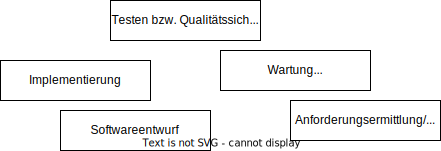
\includegraphics[scale=1.0]{Bilder/Kapitel-2/Abb-2-1.pdf}
    \caption{Kernprozesse des Softwareengineering}
    \label{fig:prozesse_softwareengineering}
\end{figure}

Die Einordnung von Prozessen und Teilprozessen in kausal-zeitliche Abfolgen ist Aufgabe von \textit{Vorgehensmodellen}. 
\marginline{von Prozessen\\zu Vorgehens\-modellen}
Im Rahmen des Softwareengineering beschreiben Vorgehensmodelle, \textbf{wie} der Entwicklungsvorgang von Softwareprodukten ablaufen soll. Je nach Zielrichtung des Vorgehensmodells werden dafür die einzelnen Prozesse und Teilprozesse des Softwareentwicklungsprozesses in bestimmter Reihenfolge und mit bestimmter Schwerpunktsetzung zusammengesetzt, wobei (Teil)Prozese auch wiederholt stattfinden können. Ergebnis ist die Definition eines idealtypisch ablaufenden Softwareentwicklungsprozesses. Für die Entwicklung eines \textbf{konkreten} Softwareprodukts müssen innerhalb des Rahmens des gewählten Vorgehensmodells dann die durchzuführenden konkreten Teilprozesse, Aktivitäten und Aufgaben für die Erstellung des Softwareprodukts bestimmt werden.

% 2.1
\clearpage
\input{Kapitel-2/Kapitel-2-1.tex}

% 2.2
\clearpage
\input{Kapitel-2/Kapitel-2-2.tex}
\input{Kapitel-2/Kapitel-2-2-1.tex}
\input{Kapitel-2/Kapitel-2-2-1-1.tex}
\input{Kapitel-2/Kapitel-2-2-2.tex}
\input{Kapitel-2/Kapitel-2-2-2-1.tex}
\input{Kapitel-2/Kapitel-2-2-3.tex}
\input{Kapitel-2/Kapitel-2-2-3-1.tex}
\input{Kapitel-2/Kapitel-2-2-3-2.tex}

% 2.3
\clearpage
\input{Kapitel-2/Kapitel-2-3.tex}

% 2.4
% Kommentierte Literatur beginnt auf neuer Seite
\clearpage
\input{Kapitel-2/Kapitel-2-4.tex}
\cleardoublepage
% Kapitel Fallbeispiel Zoo: über das Marko werden Kapitel, Eintrag Inhaltsverzeichnis und die Kopfzeilen konfiguriert.
\FallBeispielZoo
\label{sec:Lektion-1-Zoo}

Wir möchten hier am Ende dieser ersten Lektion mit einem Fallbeispiel beginnen, das Sie in den weiteren Lektionen immer mal wieder begleiten wird. Es dient dazu, aus einem praktischeren Blickwinkel ein paar Schlaglichter auf typische Tätigkeiten im Softwareengineering zu werfen. Die Simulation eines kompletten Software\-entwick\-lungs\-prozesses anhand eines Fallbeispiels ist im Rahmen einer solchen Lehrveranstaltung allerdings nicht möglich. Für das Fallbeispiel haben wir den Real\-weltbereich des Zoos gewählt und entschuldigen uns schon einmal im Vorfeld bei allen Zoo-Spezialistinnen und Zoo-Spezialisten für die Halbwahrheiten und erfundenen Informationen zur Lebenswelt Zoo in diesem natürlich für unsere Lehrzwecke so konstruierten Fallbeispiel.

\minisec{Die Ausgangslage}
Sie haben kürzlich Ihr Informatik- (wahlweise Wirtschaftsinformatik-) Studium abgeschlossen und Ihre erste Stelle in einem Unternehmen angetreten, das Softwarelösungen für kleine und mittelständische Betriebe entwickelt. Ihr neuer Chef, Herr Steiber, informiert Sie und Ihre Kolleg:innen über ein neues Projekt.

\textbf{Hr. Steiber:} „Was wissen Sie über Zoos? Wenig? Geht mir auch so. Aber das wird sich für uns alle wohl bald schon ändern: Einige von Ihnen kennen Frau Dr. Walther ja schon, die Direktorin des Zoos hier in der Stadt – und eine gute Bekannte von mir. Frau Dr. Walther ist vor einiger Zeit auf mich zugekommen, da der Zoo eine Zoo-Verwaltungssoftware benötigt. Nur, was genau gebraucht wird, in welchem Umfang, für welche Aufgaben usw. das scheint offensichtlich noch recht unklar zu sein. Frau Dr. Walther und einige ihrer Kolleginnen und Kollegen werden nächste Woche zu einem ersten Informationsgespräch bei uns vorbei kommen und ich möchte das gesamte Team bitten, dabei zu sein. Ich kann noch gar nicht einschätzen, in welchem Rahmen sich ein eventuelles Projekt bewegen würde und insofern müssen wir bei diesem ersten Gespräch auch herausfinden, inwiefern es sich für uns überhaupt lohnen würde, weitere Ressourcen zu investieren und auf eine Auftragserteilung hinzuarbeiten. Das zu lösende Problem darf einerseits natürlich nicht zu klein sein – ich sag mal, nur Eingabemasken zu erstellen, in der die Namen der Zootiere eingeben werden können, ist für uns nicht interessant. Auf der anderen Seite können wir mit unserem doch recht kleinen Team natürlich auch keine allumfassende Automatisierung sämtlicher Zooabläufe liefern - Ich fürchte ein wenig, dass es genau das ist, was der Zoo sich vorstellt. Wir werden sehen!“

\minisec{Beim ersten Treffen mit dem Zoo-Team}

\textbf{Fr. Walther (Zoodirektorin):} „Hallo. Schön, dass wir heute hier bei Ihnen sein dürfen. Herr Steiber hatte mich gebeten, etwas zu unserem Zoo zu sagen. Das ist kein Problem! Außerdem soll ich ja schon mal skizzieren, was die von uns gewünschte Zoo-Software können muss. Aber woher soll ich das wissen? Sie sind doch die Experten in der Softwareentwicklung. Sie wissen viel besser, was Softwareprodukte können müssen. Also, unser Zoo: Wir haben jährlich ca. 150.000 Besucher, im Jahresverlauf ist die Besucherzahl stark schwankend. 80 Prozent unserer Besucher sind Kinder. Natürlich hat irgendwie jedes Kind sein eigenes Lieblingstier, was sie aber alle auch mögen, ist unser Streichelzoo. Da haben wir nicht nur die üblichen Kaninchen, Meerschweinchen, Ziegen und Schafe, sondern auch unser Warzenschwein Rudi. Rudi war das erste Tier, für das wir vor ein paar Jahren die Möglichkeit eingerichtet haben, für einen jeweils begrenzten Zeitraum eine Patenschaft zu übernehmen. Mittlerweile existieren weitere Patenschaften für vier unserer Schlangen, unsere zwei Axolotl und den Kormoran. Eigentlich möchten wir das Patenschaftssystem auf alle unsere Tiere ausweiten und auch die Möglichkeit unterschiedlich langer Patenschaften bieten, aber ohne technische Unterstützung ist der Verwaltungsaufwand zu hoch. Kinder, die eine Patenschaft übernommen haben, erhalten für diesen Zeitraum freien Eintritt in den Zoo und können an bestimmten Tagen beim Füttern ihres Patentiers helfen. Wir beschäftigen fünfzehn Tierpflegerinnen und Tierpfleger und einen Tierarzt als Angestellte. Oft reicht ein Tierarzt nicht aus, sodass wir in diesen Fällen externe Tierärzte beauftragen müssen, was so kurzfristig oft nicht immer einfach ist. Wir planen langfristig eine zweite feste Tierarztstelle im Zoo einzurichten, vor allem da wir aktuell unseren Tierbestand erweitern. Bisher haben wir 26 verschiedene Tierarten mit entsprechend vielen Unterarten, \zb haben wir drei verschiedene Affenarten im Zoo. Natürlich hat jedes Tier einen Namen, und wir versuchen immer die Besucher einzubinden, wenn ein neugeborenes Tier einen Namen benötigt. Da kommt dann auch mal Shaggy raus als Name für unsere gestern geborene Testudo Graeca. Wir würden gerne alle Informationen zu unseren Tieren – also wann sie geboren sind, wer die Eltern sind, wie alt sie werden können, was sie fressen, aus welchem Zoo sie gegebenenfalls ausgeliehen sind und wie lange und ganz vieles mehr – unseren Besuchern auch über das Internet zur Verfügung stellen, aber das ist sicher aufwändig. Andererseits könnte man dann vielleicht die Eintrittskarten auch gleich online verkaufen, vielleicht würden wir dann noch mehr Besucher bekommen. Wir nutzen schon ein Onlinesystem, wenn wir Käfige oder Tiere aus anderen Zoos für eine bestimmte Zeit ausleihen und eine Software, mit der wir die Dienstpläne und Aufgaben unserer Tierpfleger verwalten, das wär schon gut, wenn das alles ein System wäre. Wir möchten langfristig nur noch fest installierte Gehege für die Tiere haben, in denen sie auch genug Platz und artgerechte Bedingungen haben, aber im Moment müssen wir auch Tiere in Käfigen halten, da sich die Bauarbeiten für die Zoo-Erweiterung verzögern. Aber wenn das mal fertig ist, werden wir endlich auch Eisbären und Nashörner haben, da fragen die Besucher nach. Seit letztem Jahr haben wir zwei Giraffen, da erhoffen wir uns dieses Jahr Nachwuchs. Tja, was müssen Sie noch wissen über unseren Zoo? Ja, genau: wir haben auch mehrere Spielplätze und natürlich Eis- und Pizzastände. Die Essensstände haben wir verpachtet. Das läuft ganz gut. Um das Essen für die Tiere kümmern sich die jeweiligen Tier\-pfleger, die kaufen entsprechend ein. Das müsste man sich auch mal angucken, ob es nicht sinnvoller wäre, die Futterbestellungen zentral zu machen, das müsste doch mit Softwareunterstützung auch viel leichter zu realisieren sein, und dann könnten wir vielleicht auch gleich noch für die Besucher im Internet Informationen über die Tierpfleger zur Verfügung stellen. Gerade unsere Stammgäste mit den Jahreskarten finden es wichtig den Tierpfleger zu kennen, der ihr Lieblingstier versorgt. Was meinen Sie, wie lange brauchen Sie für unsere Zoo-Software?“
	
	% Literaturverzeichnis für diese Lektion
	\cleardoublepage % auf einer neuen rechten Seite
	\printbibliography[heading=subbibliography]
\end{refsection}

%--- Lektion 1 --- ENDE
%----------------------------
%--- Lektion 2 --- BEGINN
\cleardoublepage
\part{Modellierung und Realwelt}
\label{sec:Lektion-2}
% wenn Änderungen zur Vorversion auf der Rückseite des Deckblatts vermerkt werden sollen, hier Auskommentierung rausnehmen 
\sttpDeckblattRueckseite{\partname~\thepart}%{\input{Lektion-2/Lektion-2-Text_fuer_Rueckseite.tex}}

\cleardoublepage
\chaptertoc % Inhaltsverzeichnis nur für diese Lektion

\begin{refsection}
	% Einbinden der einzelnen Kapitel
\cleardoublepage
\chapter*{Einleitung zur Lektion}
\addcontentsline{toc}{chapter}{Einleitung zur Lektion}
\markboth{Einleitung zur Lektion}{Einleitung zur Lektion}

Sie haben in Lektion~1 %~\ref{sec:Lektion-1}
gelernt, \marginline{das letzte Mal}
dass sich ein Softwareentwicklungsprozess aus einzelnen Prozessen (wie Anforderungsermittlung oder Implementierung) zusammensetzt, in deren Rahmen verschiedene Aktivitäten ausgeführt werden. Sie wissen zudem, dass man diesen Entwicklungsprozess auf unterschiedliche Arten strukturieren kann, indem man Vorgehensmodelle einsetzt.
 
In  dieser Lektion 
\marginline{dieses Mal}
wird wieder der Begriff \textbf{Modell} fallen. Wir werden uns mit dem Modellbegriff im Softwareengineering, mit der Realweltorientierung als zentraler Idee der Objektorientierung und darauf aufbauend mit der \textit{objektorientierten Modellierung} beschäftigen. Letztere zeichnet sich dadurch aus, dass objektorientierte Prinzipien durchgängig in den Modellierungsprozessen der Anforderungsermittlung und -analyse und des Entwurfs eingesetzt werden und nicht nur bei der Implementierung eine objektorientierte Programmiersprache verwendet wird. Auf dieser Grundlage betrachten wir die Modellierung von Realweltzusammenhängen – in der Terminologie des objektorientierten Softwareengineering als \textit{Domänenmodellierung} bezeichnet. Wir zeigen, wie sich mithilfe der Modellierungssprache UML Objekte der Realwelt, ihre Eigenschaften und Beziehungen modellieren lassen und wie die für die Objekt\-orientierung wichtigen Klassen damit in Zusammenhang stehen. Diese Lektion ist im Unterschied zu späteren noch nicht einem spezifischen Prozess des Software\-engineering gewidmet, da die Themenbereiche Objektorientierung und Modellierung alle Prozesse betreffen. Im Zuge der Domänenmodellierung werden Sie aber schon auf Verbindungen zum Prozess der Anforderungsermittlung und -analyse treffen. Wir fokussieren unseren Blick in dieser Lektion auf die Modellierung von Realweltstrukturen. Dafür benötigen wir nur wenige basale Konzepte. Die weiteren, sehr mächtigen Konzepte der Objektorientierung, die die UML auch abbilden kann, spielen für Realweltmodellierungszwecke kaum eine oder gar keine Rolle. Sie werden manche von ihnen im weiteren Verlauf des Lerntextes kennenlernen.

Schlagen 
\marginline{Bezug zu den Vorgehens\-modellen}
wir zum Schluss dieser Einleitung noch kurz den Bogen zurück zu den Vorgehensmodellen aus der letzten Lektion. Wir haben in der aktuellen Lektion – und stärker noch in den späteren Lektionen – die Situation, dass manche Aspekte des Softwareengineering, die wir darstellen, in einigen Vorgehensmodellen sehr wichtig sind und in anderen gar keine Berücksichtigung finden. Den starken Fokus auf die objektorientierte Modellierung mithilfe der UML zum Beispiel, den wir hier setzen, findet man in agilen Softwareentwicklungsprojekten häufig so nicht. In Projekten, die nach wasserfallartigem Vorgehen arbeiten, trifft man dagegen nicht selten auf den Fall, dass zwar eine objektorientierte Programmiersprache eingesetzt wird, das zentrale Konzept der Realweltorientierung der Objektorientierung (und damit auch die Domänenmodellierung) aber in den der Implementierung vorgeschalteten Prozessen vernachlässigt wird. Wir versuchen bei Aspekten, in denen sich verschiedene Arten von Vorgehensmodellen sehr stark unterscheiden, diese Problematik explizit zu machen. Sie sollten sich aber insgesamt bewusst sein, dass nicht alle Methoden, die Sie hier kennenlernen, in jedem praktischen Softwareentwicklungsprojekt eingesetzt werden. Und das hat ausnahmsweise mal nicht nur damit zu tun, dass die universitäre Ausbildung teilweise andere Schwerpunkte setzt als man sie in betrieblichen Ausbildungs- und Arbeitszusammenhängen findet.

\sttpUniversalkasten{Lernziele zu Lektion 2}{Nach dieser Lektion
	\begin{itemize}
		\item können Sie erklären, was ein Modell im Softwareengineering ist und was in diesem Zusammenhang mit dem Begriff Abstraktion gemeint ist,
		\item besitzen Sie einen ersten Einblick in die Domänenmodellierung und ihre Anwendung in unterschiedlichen Vorgehensmodellen,
		\item können Sie die Begriffe Objekt und Klasse voneinander abgrenzen und die Bedeutung von Multiplizitäten erklären,
		\item können Sie mit UML-Elementen Objekte, Klassen, ihre Eigenschaften und Beziehungen unter dem Fokus der Realweltabbildung modellieren.	
	\end{itemize}
}


%--- Kapitel 3
\chapter{Objektorientierte Modellierung}

Consetetur sadipscing elitr, sed diam nonumy eirmod tempor invidunt ut labore et dolore magna aliquyam erat, sed diam voluptua. At vero eos et accusam et justo duo dolores et ea rebum. Stet clita kasd gubergren, no sea takimata sanctus est Lorem ipsum dolor sit amet. 

\section{Modelle im Softwareengineering}

Duis autem vel eum iriure dolor in hendrerit in vulputate velit esse molestie consequat, vel illum dolore eu feugiat nulla facilisis at vero eros et accumsan et iusto odio dignissim qui blandit praesent luptatum zzril delenit augue duis dolore te feugait nulla facilisi. Lorem ipsum dolor sit amet, consectetuer adipiscing elit, sed diam nonummy nibh euismod tincidunt ut laoreet dolore magna aliquam erat volutpat.   

\section{Objektorientierung – Einführung}

Ut wisi enim ad minim veniam, quis nostrud exerci tation ullamcorper suscipit lobortis nisl ut aliquip ex ea commodo consequat. Duis autem vel eum iriure dolor in hendrerit in vulputate velit esse molestie consequat, vel illum dolore eu feugiat nulla facilisis at vero eros et accumsan et iusto odio dignissim qui blandit praesent luptatum zzril delenit augue duis dolore te feugait nulla facilisi.   

\section{Die Unified Modeling Language (UML)}

Nam liber tempor cum soluta nobis eleifend option congue nihil imperdiet doming id quod mazim placerat facer possim assum. Lorem ipsum dolor sit amet, consectetuer adipiscing elit, sed diam nonummy nibh euismod tincidunt ut laoreet dolore magna aliquam erat volutpat. Ut wisi enim ad minim veniam, quis nostrud exerci tation ullamcorper suscipit lobortis nisl ut aliquip ex ea commodo consequat.   

\newpage

\section{Objekte und Klassen – Modellierung von Realwelt-Zusammenhängen}

% 3.4.1 Objekt vs. Klasse 
\input{Kapitel-3/Kapitel-3-4-1.tex}

% 3.4.2 Eigenschaften 
\input{Kapitel-3/Kapitel-3-4-2.tex}

% 3.4.3 Verhalten
\input{Kapitel-3/Kapitel-3-4-3.tex}

%--- Kapitel 4
\cleardoublepage
\chapter{Domänenmodellierung -- Klassen und Objekte}
\label{sec:Kap-4}

Es gibt sehr viele unterschiedliche Möglichkeiten, Modelle im Softwareengineering einzusetzen. Wichtig für ein Softwareentwicklungsprojekt ist, das Modellieren nicht zum Selbstzweck werden zu lassen, sondern Modelle immer als Schritte auf dem Weg zum zu erstellenden Softwareprodukt zu sehen und somit sowohl quantitativ als auch qualitativ \textbf{zielgerichtet} zu modellieren. Das betrifft auch die Realweltmodellierung, mit der wir in diesem Kapitel beginnen. Man erstellt Modelle der Realwelt nicht, um ein hübsches Bild von den Zuständen der Wirklichkeit zu erhalten, sondern weil man ein Softwareprodukt entwickeln möchte, das \textbf{in} dieser Wirklichkeit \textbf{oder mit} dieser Wirklichkeit arbeitet.

Das Modellieren
\marginline{Modellieren ist subjektiv}
von Sachverhalten – seien es Realweltzusammenhänge oder Entwurfsentscheidungen für die Implementierung – ist stets eine subjektive Handlung. Von ganz trivialen Beispielen einmal abgesehen, können identische Sachverhalte von verschiedenen Modellierern unterschiedlich modelliert werden. Es gibt durchaus Heuristiken, an denen man sich als Modellierer orientieren kann („üblicherweise“), aber keine Formel für das ideale Diagramm. Die UML unterstützt durch die mittlerweile recht ausgereifte inhaltliche Abgrenzung ihrer unterschiedlichen Modellierungs\-elemente aber eine gewisse Standardisierung.


%--- Kapitel 4.1 - 4.3
\clearpage
\input{Kapitel-4/Kapitel-4-1.tex}

\clearpage
\input{Kapitel-4/Kapitel-4-2.tex}

\clearpage
\input{Kapitel-4/Kapitel-4-3.tex}

%--- Kapitel 4.4 KommLit
\clearpage
\input{Kapitel-4/Kapitel-4-4.tex}

%Zoo
\cleardoublepage
% Kapitel Fallbeispiel Zoo: über das Marko werden Kapitel, Eintrag Inhaltsverzeichnis und die Kopfzeilen konfiguriert.
\FallBeispielZoo
\label{sec:Lektion-2-Zoo}

\marginline{~\\Lektion~1, Seite~\pageref*{sec:Lektion-1-Zoo}}
\sttpUniversalkasten{Was bisher geschah}{Der städtische Zoo ist an das Softwareunternehmen herangetreten, in dem Sie arbeiten, um zu eruieren, an welchen Stellen Zooabläufe mit Software unterstützt werden könnten und wie der öffentliche Zooauftritt insgesamt digitaler werden kann. Welche Dienstleistungen der Zoo von Ihrem Unternehmen erwartet, ist aktuell noch recht vage. \newline \newline	
Wir befinden uns in einer ersten Brainstorming-Besprechung zwischen dem Softwareentwicklungsteam und einer Abordnung des Zoos. Frau Dr. Walther, die Zoodirektorin, hat soeben in einem sehr informationsdichten Rundumschlag zur Domäne Zoo erzählt und dabei auch erste Andeutungen gemacht, für welche Aspekte sie sich Softwareunterstützung vorstellen könnte.}

\minisec{Die Besprechung wird fortgesetzt}

Ihr Chef, Herr Steiber, bedankt sich bei der Zoodirektorin für ihre Ausführungen. Im Anschluss wird frei diskutiert, es wird nachgefragt, zusätzliche Informationen werden erteilt, Unklarheiten angesprochen, manches konkretisiert, anderes im Vagen gelassen, weitere Wünsche geäußert, jede und jeder macht sich ein paar Notizen,~\ldots 
\linebreak
Auf diese Weise sind schnell zwei Stunden vergangen. Die Chemie scheint zu stimmen zwischen dem Zoo- und dem Softwareentwicklungsteam.

Herr Steiber und die Zoodirektorin haben dann auch zwischenzeitlich eine Kaffeepause genutzt, um sich grundsätzlich auf die Zusammenarbeit zu verständigen. Man definiert die heutige Besprechung als Beginn eines kleineren Vorprojekts, in dem der inhaltliche und zeitliche Rahmen für das hoffentlich anschließende eigentliche Softwareentwicklungsprojekt verhandelt wird. Herr Steiber konnte der Zoo\-direk\-torin auch schon mal vorsichtig nahebringen, dass es sicher nicht auf eine allumfassende vollintegrierte und automatisierte Zooverwaltungs- und Zoodigitalisierungssoftware hinauslaufen wird.

\textbf{Hr. Steiber:} „Ich darf um Ihre Aufmerksamkeit bitten! Schön, dass wir schon so intensiv ins Diskutieren gekommen sind. Wir sollten unseren Austausch jetzt aber etwas systematisieren und vor allem unsere Gedanken festhalten. Daher bitte ich Sie, auf den Karteikarten die noch offenen Fragen zur Domäne zu notieren. Erstellen Sie dort bitte auch kurze Beschreibungen der Zoo-Abläufe und -Aufgaben, über die wir hier gerade diskutiert hatten. Einige von Ihnen hatten sich vorhin zudem schon erste Gedanken über das zukünftige Softwareprodukt gemacht, halten Sie das bitte auch alles auf den Karteikarten fest. Und Kollege Fryt, beginnen Sie doch bitte parallel schon mal mit einem ersten groben Domänenklassendiagramm, Sie sehen ja, welche Informationen zur Domäne die anderen ans Whiteboard heften. Aber verlieren Sie sich bloß noch nicht im Detail, da wird es sicher noch viele Änderungen geben, wenn wir uns weiter über die Domäne austauschen.“

\minisec{Einige Zeit später}

% Anmerkung: man kann die Verweise noch wie gewünscht anpassen. Wenn der Verweis hinter den Grafiken stört (roter Rahmen), dann nimmt man "\hyperref[...]{}" weg und lässt nur den 2. Parameter in der geschweiften Klammer stehen. Bei den Bildunterschriften kann man ebenfalls frei entscheiden, wie es aussehen soll.

\begin{center}
	\begin{minipage}[c]{.65\linewidth}
		\centering
		\hyperref[text:lektion2_whiteboard_s1]{\includegraphics[width=0.45\linewidth]{Bilder/Zoo/whiteboard_s1.png} \includegraphics[width=0.45\linewidth]{Bilder/Zoo/whiteboard_s2.png}}
		Whiteboard mit Karteikarten (vergrößerte Darstellung auf Seite~\pageref{text:lektion2_whiteboard_s1}f.)
	\end{minipage}
	\hspace{0.1cm}% Abstand zwischen den beiden Bildern
	\begin{minipage}[c]{.33\linewidth}
		\centering
		\hyperref[fig:lektion2_fallbeispiel_zoo]{\includegraphics[width=\linewidth]{Bilder/Zoo/fallbeispiel_zoo.pdf}}
		Domänenklassendiagramm Zoo (vergrößert in Abbildung~\ref{fig:lektion2_fallbeispiel_zoo})
	\end{minipage}
\end{center}

\textbf{Hr. Steiber:} „Ich danke Ihnen allen! Für das erste Treffen waren wir doch schon sehr produktiv. Sie haben ja schon mitbekommen, dass mit diesem Treffen unser Vorprojekt nun offiziell gestartet ist. Wir werden uns in den nächsten Tagen und Wochen in kleineren Runden wieder treffen und zum einen an der Modellierung der Domäne weiterarbeiten und zum anderen uns natürlich über den Inhalt des zu entwickelnden Softwareprodukts Gedanken machen. Die Kollegin Schwab wird als sehr erfahrene Projektleiterin die Leitung des Vorprojekts übernehmen und zeitnah die verschiedenen Arbeitsgruppen einteilen. Für heute beende ich die Besprechung und wünsche uns allen einen schönen Feierabend.“

\minisec{Am nächsten Tag im Softwareunternehmen}
Die drei Kolleg:innen Inga Schwab (Projektleiterin Vorprojekt), Magnus Fryt (Requirement Engineer) und Joris Jonson (Softwarearchitekt) sitzen zusammen und planen die nächsten Schritte.

\textbf{Inga Schwab:} „Die Domäne Zoo ist komplexer, als ich das gedacht hatte. Unser aktuelles Domänenmodell ist noch viel zu grob. Lasst uns zunächst mal bei der Klasse Tier und der Klasse Tierpfleger ansetzen. Diese Informationen werden wir in jedem Fall brauchen, unabhängig davon, auf welche Aufgabenbereiche für das Softwareprodukt wir uns einigen. Tier scheint nicht gleich Tier zu sein. Ich habe den Eindruck, dass Strukturen und Abläufe der Domäne durchaus unterschiedlich aussehen, je nachdem über welche Tierart wir sprechen. Und auch bei den Tier\-pflegern scheinen Arbeitsabläufe davon abhängig zu sein, welche Tierarten sie betreuen. Was mir gestern, trotz der umfangreichen Erklärungsversuche des Zoo-Teams, bis zum Schluss nicht klar geworden ist, warum es einen auf Löwen spezialisierten Tier\-pfleger geben muss und einen anderen Tierpfleger für die Tiger, die Nagetiere und die Fische aber vom selben Tierpfleger versorgt werden können. Möglicherweise ist das nur historisch so gewachsen im Zoo, aber wir müssen sicher sein, dass uns hier nicht grundlegende Restriktionen der Domäne entgehen. Magnus, übernimm du bitte die Leitung der Arbeitsgruppe Domänenmodellierung. Hol dir Paul dazu, er hat sich in der Besprechung gestern schon gut in die Domäne herein gedacht. Von der Zooseite aus versuche ich dir zwei bis drei der Tierpfleger für die Arbeitsgruppe zu organisieren. Joris, du und ich werden uns mit der Zoo-Führung zusammensetzen und in die Entwicklungsplanung einsteigen, erste Prioritäten hat Frau Dr. Walther ja gestern immerhin schon gesetzt.“

% Das Whiteboard wird auf 2 Seiten dargestellt und soll somit auf einer linken Seite beginnen.
\cleardoubleevenemptypage 

\input{Lektion-2/Lektion-2-Whiteboard-Seite1.tex}

\clearpage

\input{Lektion-2/Lektion-2-Whiteboard-Seite2.tex}

\clearpage

\vspace*{4cm} %%% Abbildung auf Seite zentrieren

\begin{figure}[h!]
	\centering
	\includegraphics{Bilder/Zoo/fallbeispiel_zoo.pdf}
	\caption{Domänenklassendiagramm für den Zoo}
	\label{fig:lektion2_fallbeispiel_zoo}
\end{figure}

	
	% Literaturverzeichnis für diese Lektion
	\cleardoublepage % auf einer neuen rechten Seite
	\printbibliography[heading=subbibliography]
\end{refsection}

%--- Lektion 2 --- ENDE
%----------------------------
%--- Lektion 3 --- BEGINN
\cleardoublepage
\part{Prozessmodellierung mit Petrinetzen}
\label{sec:Lektion-3}
% wenn Änderungen zur Vorversion auf der Rückseite des Deckblatts vermerkt werden sollen, hier Auskommentierung rausnehmen
\sttpDeckblattRueckseite{\partname~\thepart}%{\input{Lektion-3/Lektion-3-Text_fuer_Rueckseite.tex}}

\cleardoublepage
\chaptertoc % Inhaltsverzeichnis nur für diese Lektion

\begin{refsection}
	%% Einbinden der einzelnen Kapitel
\cleardoublepage
\chapter*{Vorwort}
\addcontentsline{toc}{chapter}{Vorwort}
\markboth{Vorwort}{Vorwort}

Diese Lektion wurde zum Sommersemester 2024 in Form einer Video-Vorlesungs\-reihe konzipiert, die Sie im Moodleauftritt des Moduls finden. Die Entscheidung für Videos begründete sich auf dem Wunsch vieler Studierender audiovisuelle Lernmaterialien nutzen zu können, vor allem aber in der besseren Darstellbarkeit von Prozessen und ihren Modellen, die im Videoformat Schritt-für-Schritt entwickelt und erklärt werden können. Nutzen Sie die Möglichkeit die Video-Vorlesungen zu verfolgen, um ein umfassendes Verständnis der behandelten Konzepte zu erlangen. Diese textuelle Version enthält zwar auch die meisten Inhalte aus den Vorlesungen, behandelt die Themen allerdings weniger ausführlich.

Hinweis: In diesem Kapitel werden Ihnen an vielen Stellen formale Beweise begegnen. Das Verständnis, aber auch die eigene Formulierung von Beweisen sowie die Anwendung formaler Methoden sind grundlegend für die Entwicklung zuverlässiger und fehlerfreier Software und eine wichtige Kernkompetenz im Softwareengineering. Befassen Sie sich also intensiv damit – nicht nur, weil es erwartet wird, sondern auch, weil es Ihnen letztlich tatsächlich nützen wird. Die Übungs- und Einsendeaufgaben zu dieser Lektion sind ein Anhaltspunkt dafür, wann wir eigene Beweise von Ihnen erwarten und wann das Verstehen der Beweise aus der Vorlesung bzw. aus diesem Text ausreicht.
\cleardoublepage
\chapter*{Einleitung zur Lektion}
\addcontentsline{toc}{chapter}{Einleitung zur Lektion}
\markboth{Einleitung zur Lektion}{Einleitung zur Lektion}

In Lektion 2 haben wir die Grundprinzipien der Modellierung vorgestellt,  
\marginline{Modell und Veränderung}
basierend auf der Definition von Herbert Stachowiak: Modelle sind Abstraktionen natürlicher oder künstlicher Originale, deren Eigenschaften vereinfacht dargestellt oder weggelassen werden, um innerhalb eines Geltungsbereichs für eine bestimmte Zielgruppe spezifische Zwecke zu erfüllen. Auf diesem Verständnis aufbauend haben Sie die Modellierungssprache UML kennengelernt und in Objekt- und Klassendiagrammen strukturelle Aspekte der Realwelt visualisiert. Dabei haben Sie gesehen, dass sich die Objekte der Klassen ändern können: Es können Objekte erzeugt werden, es können sich Attributwerte und damit Objektzustände verändern, Verbindungen können hinzugefügt oder gelöscht werden. Dies geschieht natürlich, weil entsprechende Veränderungen der Realwelt abgebildet werden sollen. Und insbesondere auch, weil dies Auswirkungen der Abläufe sind, die unsere Software realisieren soll.

Klassendiagramme formulieren Regeln, die immer gelten, 
\marginline{Modellierung von Verhalten}
während zugehörige Objektkonstellationen nur für einen bestimmten Zeitpunkt gelten, also Momentaufnahmen eines eventuell komplexen und verteilten Systems darstellen. Die Konstellationen von Objekten können sich auf vielfältige Weise ändern, doch sind diese Änderungen nicht beliebig und nicht unabhängig voneinander, weil ansonsten die genannten Regeln verletzt werden können. Mögliche Änderungen werden durch das Verhalten von Systemen und Prozessen (den Unterschied werden Sie später kennenlernen) beschrieben, und auch dafür braucht es Modelle. Diese Lektion behandelt die Modellierung von Verhalten. Wir werden Modelle zum Verständnis von Verhalten in der Realwelt einsetzen, aber auch zur Beschreibung des Verhaltens von Software.

Prozessmodellierung, 
\marginline{Prozess\-modellierung}
wie sie Ihnen im professionellen Kontext und in der Literatur begegnet, findet Anwendung sowohl in der Informatik als auch in der Wirt\-schafts\-infor\-matik (sie spielt dort insbesondere bei der Optimierung von Geschäftsprozessen eine Rolle). Sie lässt sich also im interdisziplinären Kontext dieser beiden Disziplinen verorten. Seit den späten 1970er Jahren haben sich viele verschiedene Modellierungssprachen für Prozesse entwickelt. Diese Sprachen variieren in ihren spezifischen Ausdrucksformen und Schwerpunkten. In unserer Lehrveranstaltung verwenden wir Petrinetze für die Prozessmodellierung.

\pagebreak %%% für Druck

\sttpAutorenkasten{Carl Adam Petri}{1926}{2010}{Deutscher Mathematiker und Informatiker. Leitete ein Institut der Gesellschaft für Mathematik und Datenverarbeitung (GMD) in St. Augustin bei Bonn. Bekannt ist er vor allem für die nach ihm benannten Petrinetze zur Modellierung des Verhaltens verteilter Systeme.}{Bilder/Autoren/petri.jpg}{2009}{Michael Krapp, \href{http://creativecommons.org/licenses/by-sa/3.0}{CC BY-SA 3.0}, via \href{https://commons.wikimedia.org/wiki/File:Carl_adam_petri.jpg}{Wikimedia Commons}}

\vspace{-1ex} %%% für Druck

\subsection*{Warum Petrinetze?}

\textbf{Petrinetze als Grundlage für andere Prozess-Modellierungssprachen}\\
Obwohl Petrinetze in der praktischen Anwendung möglicherweise nicht (mehr) weit verbreitet sind, bilden sie die theoretische Grundlage für beinahe alle anderen Pro\-zess-Model\-lie\-rungs\-tech\-niken und -sprachen.

\textbf{Einfache Visualisierung}\\
Petrinetze verfügen über eine leicht erlernbare und verständliche grafische Darstellungsform, die nur wenige unterschiedliche Elemente beinhaltet.

\textbf{Modellierung verteilter Systeme mit verteilten, lokalen Zuständen}\\
In verteilten Systemen führen die möglichen Kombinationen der lokalen Zustände der Komponenten zu einer exponentiellen Zunahme möglicher globaler Zustände. Petrinetze bewältigen diese Komplexität, indem globale Zustände nicht explizit modelliert werden, sondern sich aus den Kombinationen der lokalen Zustände ergeben. So wächst die Größe eines Petrinetzes nur linear mit der Systemgröße, was eine effi\-zi\-ente und doch präzise Modellierung großer Systeme ermöglicht. Diese Art der Modellierung hat nicht nur den Vorteil die Komplexität des Modells überschaubar zu halten, sondern spiegelt auch die modulare Struktur des modellierten Systems wider.

\textbf{Präzise Darstellung des Verhaltens von Systemkomponenten}\\
Die Modellierung komplexer Prozesse in der Softwareentwicklung mithilfe von Petrinetzen erlaubt ein tiefes Verständnis für die Dynamik und Interaktion von Systemkomponenten, denn die Abläufe eines Prozesses und auch seiner Komponenten sowie ihre Eigenschaften und deren Beziehungen zueinander sind formal definiert und können präzise dargestellt werden.

\textbf{Mathematische Basis}\\
Die mathematische Grundlage der Petrinetze ermöglicht es Modelle systematisch und auch automatisch (mit entsprechenden Werkzeugen) auf Korrektheit und Konsistenz zu überprüfen. Auf diese Weise können Fehler in der Programmlogik eines modellierten Systems bereits frühzeitig erkannt und behoben werden, noch bevor sie beim Testen oder im laufenden Betrieb auftreten. In den vergangenen 60 Jahren wurde eine Vielzahl von Algorithmen entwickelt, und entsprechende Werkzeuge stehen zur Verfügung.

\textbf{Nebenläufigkeit als Konzept}\\
Ein weiterer wesentlicher Vorteil von Petrinetzen ist die kausale, nicht-sequentielle Interpretation von Abläufen. Wie Sie im Laufe dieses Kapitels verstehen werden, entspricht dies in den meisten Fällen der Realität, in der Aktivitäten unabhängig voneinander stattfinden. Diese Philosophie mag zunächst ungewohnt erscheinen, ist jedoch äußerst wertvoll. Sobald Sie sie verstanden haben, kann sie Ihnen in vielen anderen Bereichen nützlich sein.

\sttpUniversalkasten{Lernziele zu Lektion 3}{Nach dieser Lektion
	\begin{itemize}
		\item können Sie die Begriffe System, Prozess, Prozessablauf im Modellierungskontext erklären und voneinander abgrenzen.
		\item können Sie Petrinetzmodelle für einfache Systeme und Prozesse erstellen und verstehen Sie, wie derartige Modelle durch Methoden des Process Mining und der Synthese entstehen.
		\item verstehen Sie zentrale Eigenschaften von Systemen und Prozessen und wissen, wie man diese formal definiert und für gegebene Beispiele prüft.
		\item können Sie Theoreme und Beweise zu komplexeren mathematisch formulierten Beziehungen zwischen Modelleigenschaften nachvollziehen und für einfachere Beziehungen selbst erstellen.
		\item kennen Sie verschiedene praxisrelevante Sprachen für die Modellierung von Prozessen und Systemverhalten, insbesondere aus der UML, und können die Bezüge zu Petrinetzen erläutern.
	\end{itemize}
}

%%--- Kapitel 5
%--- Kapitel 5
\cleardoublepage
\chapter{Prozessmodellierung mit Petrinetzen}
\label{sec:Kap-5}

%--- Kapitel 5.1 - 5.12
% \clearpage Hier keinen Seitenumbruch!
\input{Kapitel-5/Kapitel-5-1.tex}
\clearpage
\input{Kapitel-5/Kapitel-5-2.tex}
\clearpage
\input{Kapitel-5/Kapitel-5-3.tex}
\clearpage
\input{Kapitel-5/Kapitel-5-4.tex}
\clearpage
\input{Kapitel-5/Kapitel-5-5.tex}
\clearpage
\input{Kapitel-5/Kapitel-5-6.tex}
\clearpage
\input{Kapitel-5/Kapitel-5-7.tex}
\clearpage
\input{Kapitel-5/Kapitel-5-8.tex}
\clearpage
\input{Kapitel-5/Kapitel-5-9.tex}
\clearpage
\input{Kapitel-5/Kapitel-5-10.tex}
\clearpage
\input{Kapitel-5/Kapitel-5-11.tex}

% 5.12
% Kommentierte Literatur beginnt auf neuer Seite
\clearpage
\input{Kapitel-5/Kapitel-5-12.tex}

	
	% Literaturverzeichnis für diese Lektion
	\cleardoublepage % auf einer neuen rechten Seite
	\printbibliography[heading=subbibliography]
\end{refsection}

%--- Lektion 3 --- ENDE
%----------------------------
%--- Lektion 4 --- BEGINN
\cleardoublepage
\part{Requirements Engineering}
\label{sec:Lektion-4}
% wenn Änderungen zur Vorversion auf der Rückseite des Deckblatts vermerkt werden sollen, hier Auskommentierung rausnehmen 
\sttpDeckblattRueckseite{\partname~\thepart}%{\input{Lektion-4/Lektion-4-Text_fuer_Rueckseite.tex}}

\cleardoublepage
\chaptertoc % Inhaltsverzeichnis nur für diese Lektion

\begin{refsection}
	% Einbinden der einzelnen Kapitel
\cleardoublepage
\chapter*{Einleitung zur Lektion}
\addcontentsline{toc}{chapter}{Einleitung zur Lektion}
\markboth{Einleitung zur Lektion}{Einleitung zur Lektion}

In \marginline{diese Lektion und die vorherigen} Lektion~1 % todo Lektion~\ref{sec:Lektion-1}
hatten Sie schon einen ersten Überblick über die Kernprozesse des Softwareengineering erhalten. Ab dieser Lektion werden wir uns mit diesen Kernprozessen detaillierter beschäftigen. Dabei werden Ihnen auch die Vorgehensmodelle aus Lektion~1 % todo Lektion~\ref{sec:Lektion-1} 
regelmäßig wieder begegnen. Ebenso wird Sie und uns der Modell\-begriff aus Lektion~2 % todo Lektion~\ref{sec:Lektion-2}
weiter beschäftigen. Die Modellierung der Realwelt wird über die Domänenmodellierung als Aktivität innerhalb der Anforderungsermittlung wieder Thema sein. Und schließlich haben Sie in Lektion~3 gelernt, dass nicht nur Zusammenhänge zwischen Objekten der Realwelt modelliert werden, sondern dass auch ihr Verhalten und ihr Zusammenspiel Gegenstand der Modellierung ist, und dass dies, je nach Betrachtungswinkel, mit verschiedenen Modellierungssprachen möglich ist. Ab dieser Lektion werden uns die Blickwinkel Struktur und Verhalten zunehmend nicht mehr nur bezogen auf den Modellierungsgegenstand Realwelt sondern vor allem auf den Modellierungsgegenstand (zukünftiges) Softwareprodukt beschäftigen.

In \marginline{Kernprozesse} einem Softwareentwicklungsprozess spezifiziert man die Anforderungen an das zukünftige Softwareprodukt, überlegt sich dessen Struktur, implementiert und testet es. Sofern man agil vorgeht, spezifiziert man zunächst nur einen Teil der Anforderungen, verzichtet vielleicht auf einen dokumentierten Softwareentwurf und verzahnt stattdessen Entwurfs- und Implementierungstätigkeiten, testet -- möglicherweise hat man die Tests schon pa\-ra\-llel zu den Anforderungen aufgeschrieben, noch bevor man mit der Implementierung beginnt -- und startet die nächste Iteration. Die vier \mbox{Schritte} \textbf{spezifizieren, entwerfen, implementieren und testen} findet man in jedem Softwareentwicklungsprozess, unabhängig davon, nach welchem Vorgehensmodell, in welcher Reihenfolge und mit welchen Methoden gearbeitet wird. Diese Lektion beschäftigt sich mit dem Spezifizieren. Die anderen drei Schritte werden in den folgenden drei Lektionen behandelt.

Das \marginline{Requirements Engineering} Thema dieser Lektion ist somit der Umgang mit Anforderungen im Rahmen des Softwareengineering. Der englische Begriff für diesen Themenkomplex ist Requirements Engineering. Analog zum Begriff Softwareengineering soll mit \textit{Requirements Engineering} der \textbf{ingenieurmäßige, systematische Umgang} mit Anforderungen betont werden. Der Prozess des Requirements Engineering ist ein Kernprozess des Softwareengineering und umfasst die Ermittlung und Dokumentation von Anforderungen, die Prüfung und Anpassung von erfassten Anforderungen, aber auch verschiedene Aktivitäten zur Verwaltung von Anforderungen sowie zum Umgang mit Anforderungsänderungen. Einen so umfassenden deutschen Begriff wie das englische Requirements Engineering gibt es nicht. Der sich unter Umständen anbietende Begriff Anforderungsmanagement ist in der deutschen Literatur enger besetzt, indem er nur die Themenbereiche Anforderungsverwaltung und Anforderungs\-änderung adressiert. Wenn man einen deutschsprachigen Begriff verwenden möchte, wählt man meistens die Begriffskombination „Anforderungsermittlung/-analyse“ als Übersetzung für Requirements Engineering. Diesen Weg sind auch wir in den bisherigen Lektionen gegangen. Dabei bleibt aber häufig unklar, ob alle Aspekte des Umgangs mit Anforderungen gemeint sind oder nur Teilprozesse. Daher hat sich der englische Begriff Requirements Engineering auch in der deutschsprachigen Literatur etabliert. Ab dieser Lektion, in der wir uns das erste Mal systematischer mit Anforderungen beschäftigen, werden wir ihn nun ebenfalls verwenden.

\sttpUniversalkasten{Lernziele zu Lektion 4}{Nach dieser Lektion
	\begin{itemize}
		\item können Sie die Begriffe Stakeholder, Vision, Ziele, Produktumfang und Systemkontext erläutern, sie gegeneinander abgrenzen sowie sie in einen Zusammenhang zum Begriff Anforderung setzen,
		\item kennen Sie Quellen und Kategorisierungen von Anforderungen und können erklären, was Nutzeranforderungen, Systemanforderungen, domänenbasierte Anforderungen, funktionale Anforderungen und nichtfunktionale Anforderungen sind,
		\item kennen Sie die Teilprozesse des Requirements Engineering und können ihr Zusammenspiel erläutern,
		\item können Sie über das UML-Anwendungsfalldiagramm Produkt\-anforde\-rungen und Domänenaspekte modellieren.	
	\end{itemize}
}

%--- Kapitel 6
%--- Kapitel 6
\cleardoublepage
\chapter{Requirements Engineering}
\label{sec:Kap-6}

Seit Anfang der 2000er Jahre erhält der Prozess des Requirements Engineering 
\marginline{Bedeutung des Requirements Engineering}
innerhalb des Softwareengineering-Umfelds eine stark wachsende Aufmerksamkeit. Das hat sicher auch damit zu tun, dass Studien seit dieser Zeit ungenügendes Require\-ments Engineering als einen der Hauptgründe für das Scheitern von Software\-entwicklungs\-projekten identifizieren. Bei \cite[4]{ebe22} finden Sie Verweise auf entsprechende Studien der 2000er bis 2020er Jahre. 

\phantomsection
\label{sec:Kap-6:IREB}
2006 gründeten internationale Softwareengineering-Expertinnen und -Experten von Industrieunternehmen, Beratungsdienstleistern, Universitäten und Fachhochschulen das „International Requirements Engineering Board (IREB)“ (\href{https://www.ireb.org}{www.ireb.org}) mit dem Ziel, den Prozess des Requirements Engineering zu professionalisieren. IREB ist eine Non-Profit-Organisation, die mittlerweile eine wichtige Rolle bei der Standardisierung von Begriffen und Aktivitäten des Requirements Engineering einnimmt. Dazu hat auch beigetragen, dass IREB mit dem „Certified Professional for Require\-ments Engineering \mbox{(CPRE)}“ ein Zertifizierungsprogramm anbietet, das von vielen Unternehmen zur Weiterbildung ihrer Mitarbeiterinnen und Mitarbeiter genutzt wird. Der Fokus von CPRE liegt auf der Vermittlung von in der Praxis relevanten und bewährten Methoden des Requirements Engineering.

Es gibt außerordentlich viel Literatur 
\marginline{Literatur}
zum Thema Requirements Engineering, neben den entsprechenden Kapiteln in Softwareengineering-Lehrbüchern und -Handbüchern auch sehr viele explizit nur dem Requirements Engineering gewidmete Mono\-graphien sowie zahlreiche Zeitschriftenartikel zu einzelnen Aspekten des Themas. Ganz grob lassen sich zwei Kategorien von Autoren unterscheiden -- wobei es natürlich auch Schnittmengen gibt. Zum einen diejenigen, die sich im Umfeld von Universitäten, Fachhochschulen oder Forschungseinrichtungen bewegen und Methoden des Requirements Engineering unter Lehr- oder Forschungsaspekten in einem größeren Kontext betrachten. Zum anderen diejenigen, die Unternehmen und Projekte zum Thema Require\-ments Engineering beraten und schulen und dessen Methoden sehr praxisnah mit Checklisten, Schablonen, Erfahrungswerten etc. vermitteln.

Beide Ansätze haben ihre Vor- und Nachteile. Gerade für Anfänger des Requirements Engineering lohnt es sich, Literatur aus beiden Kategorien zu lesen. Beiden Literaturkategorien gemeinsam ist, dass fast jeder Autor / jede Autorin seine / ihre eigenen Schwerpunkte setzt und damit in verschiedener Literatur häufig unterschiedliche Methoden für den Umgang mit Anforderungen vorgestellt werden. Das hat insofern seine Berechtigung als für unterschiedliche Software\-entwicklungs\-projekte, Teams und Domänen durchaus unterschiedliche Methoden jeweils besser geeignet sein können, beruht aber natürlich auch auf Vorlieben der Vorstellenden. 

Alle Inhalte und Methoden des Requirements Engineering im Detail hier im Modul vorzustellen ist nicht möglich, und auch nicht sinnvoll. Wir orientieren uns für die Struktur dieses Kapitels überwiegend an SWEBOK und an dem IREB-Standard. Frei von Vorlieben ist unsere Auswahl selbstverständlich auch nicht. Weiterführende Literaturverweise finden Sie in dieser Lektion außer am Ende des Kapitels auch schon eingestreut in die inhaltlichen Abschnitte.

\vspace{\baselineskip} %%% für Druck

\begin{figure}[h!]
	\centering
	\includegraphics[width=\textwidth]{Bilder/Kapitel-6/aktivitaeten_requirements_engineering.pdf}
	\caption{Teilprozesse des Requirements Engineering}
	\label{fig:aktivitaeten_requirements_engineering}
\end{figure}

\vspace{\baselineskip} %%% für Druck

Der Prozess des Requirements Engineering kann in die vier Teilprozesse "`Anforderungsermittlung"', "`Erstellung der Anforderungsspezifikation"', "`Anforderungs-
\linebreak %%% für Druck
validierung"' und "`Anforderungsmanagement"' unterteilt werden (s.~Abb.~\ref{fig:aktivitaeten_requirements_engineering}). In allen vier Teilprozessen kommt der Begriff \textit{Anforderung} vor.

Abschnitt~\ref{sec:Kap-6.2} wird sich nachher detaillierter mit Anforderungen, ihren Quellen, ihren Beziehungen und den Möglichkeiten, sie zu kategorisieren, beschäftigen. An dieser Stelle sagen wir erstmal allgemein: \marginline{Anforderung}
Eine Anforderung ist etwas, das \textbf{„jemand“} von dem (zukünftigen) Softwareprodukt erwartet, um ein bestimmtes Problem lösen oder ein bestimmtes Ziel erreichen zu können. Und wir beginnen dieses Kapitel mit dem „jemand“, die oder der eine Anforderung stellt -- dem sogenannten Stakeholder.



% 6.1
\clearpage
\input{Kapitel-6/Kapitel-6-1.tex}
\input{Kapitel-6/Kapitel-6-1-1.tex}
\input{Kapitel-6/Kapitel-6-1-2.tex}
\input{Kapitel-6/Kapitel-6-1-2-1.tex}
\input{Kapitel-6/Kapitel-6-1-2-2.tex}
\input{Kapitel-6/Kapitel-6-1-3.tex}
\input{Kapitel-6/Kapitel-6-1-3-1.tex}
\input{Kapitel-6/Kapitel-6-1-3-2.tex}
\newpage
\input{Kapitel-6/Kapitel-6-1-4_zoo.tex}
% 6.2
\clearpage
% ACHTUNG: im nächsten Abschnitt explizit mit "\markboth" die Texte für die Kopfzeilen neu setzen, da diese nach "Zoo" kaputt sind.
\input{Kapitel-6/Kapitel-6-2.tex}
\input{Kapitel-6/Kapitel-6-2-1.tex}
\input{Kapitel-6/Kapitel-6-2-2.tex}
\input{Kapitel-6/Kapitel-6-2-3.tex}
\input{Kapitel-6/Kapitel-6-2-4.tex}
% 6.3
\clearpage
\input{Kapitel-6/Kapitel-6-3.tex}
\input{Kapitel-6/Kapitel-6-3-1.tex}
\input{Kapitel-6/Kapitel-6-3-2.tex}
% 6.4
\clearpage
\input{Kapitel-6/Kapitel-6-4.tex}
\input{Kapitel-6/Kapitel-6-4-1.tex}
\input{Kapitel-6/Kapitel-6-4-2.tex}
\input{Kapitel-6/Kapitel-6-4-3.tex}
\input{Kapitel-6/Kapitel-6-4-4.tex}
% 6.5
\clearpage
\input{Kapitel-6/Kapitel-6-5.tex}
% 6.6 kommentierte Literatur
\clearpage
\input{Kapitel-6/Kapitel-6-6.tex}
	
	% Literaturverzeichnis für diese Lektion
	\cleardoublepage % auf einer neuen rechten Seite
	\printbibliography[heading=subbibliography]
\end{refsection}

%--- Lektion 4 --- ENDE
%----------------------------
%--- Lektion 5 --- BEGINN
\cleardoublepage
\part{Entwurf}
\label{sec:Lektion-5}
% wenn Änderungen zur Vorversion auf der Rückseite des Deckblatts vermerkt werden sollen, hier Auskommentierung rausnehmen 
\sttpDeckblattRueckseite{\partname~\thepart}%{\input{Lektion-5/Lektion-5-Text_fuer_Rueckseite.tex}}

\cleardoublepage
\chaptertoc % Inhaltsverzeichnis nur für diese Lektion

\begin{refsection}
	% Einbinden der einzelnen Kapitel
\cleardoublepage
\chapter*{Einleitung zur Lektion}
\addcontentsline{toc}{chapter}{Einleitung zur Lektion}
\markboth{Einleitung zur Lektion}{Einleitung zur Lektion}

Diese Lektion beschäftigt sich mit dem Kernprozess \textbf{Entwurf} des Software-
\linebreak %%% für Druck
engineering. Auch beim Entwurf geht es wieder um Modellierung. Der Modellierungs\-gegenstand ist nun in erster Linie das zu entwickelnde Softwaresystem. Domänen\-objekte, die zu Objekten im System werden sollen, spielen jedoch weiterhin eine große Rolle. Die Domänenmodellierung als Ganzes ist aber nur noch dann relevant, wenn den Ergebnissen aus dem Requirements Engineering die notwendige Ausdifferenzierung fehlt, um konkrete Klassen für den späteren Programmcode zu spezifizieren, oder wenn sie sich als inkonsistent herausgestellt haben. 

Wichtige Aufgaben im Rahmen des Entwurfs sind die Festlegung der Software\-architektur sowie die Bestimmung der einzelnen Komponenten des Software\-systems und deren Schnittstellen. Eine weitere Aufgabe ist der Entwurf für die Daten\-haltung/""Datenbank. Diese behandeln wir in diesem Modul nicht, hierfür gibt es eigene \mbox{Module}. 

Diese Lektion besteht aus zwei Kapiteln. Kapitel~\ref{sec:Kap-7} behandelt das Thema Software\-architektur und betrachtet damit das zukünftige Softwaresystem auf einer hohen Abstraktions\-ebene. Kapitel~\ref{sec:Kap-8} beschäftigt sich auf einer niedrigen Abstraktions\-ebene mit Klassen und Objekten im Kontext des Entwurfs. Das Thema Entwurfs\-prinzipien, das wir mit in Kapitel~7 platziert haben, verbindet diese beiden sowie die Abstraktionsebenen dazwischen.

\clearpage

\sttpUniversalkasten{Lernziele zu Lektion 5}{Nach dieser Lektion
	\begin{itemize}
		\item wissen Sie, was eine Softwarearchitektur ist und kennen wichtige Faktoren für ihre Auswahl und Ausgestaltung,
		\item können Sie erklären, was Architekturmuster sind und wozu diese gut sind. Sie kennen die Schichtenarchitektur und Client-Server-Architekturen als Beispiele für Architekturmuster und können deren grundsätzliche Funktions\-weise erläutern,
		\item können Sie erklären, was Entwurfsprinzipien sind. Sie kennen die grundsätzlichen Einsatzzwecke der in der Lektion vorgestellten Entwurfs\-prinzipien und die Unterschiede zwischen ihnen,
		\item können Sie erklären, in welchen Zusammenhängen und mit welchen \mbox{Bedeutungen} die Begriffe Komponente und Schnittstelle im Rahmen des Software\-entwurfs verwendet werden,
		\item können Sie mit Elementen des UML-Klassendiagramms Klassen, ihre Eigen\-schaften, ihr Verhalten und ihre Beziehungen mit dem Fokus auf Softwareentwurf modellieren.		
	\end{itemize}
}

%--- Kapitel 7
%--- Kapitel 7
\cleardoublepage
\chapter{Softwarearchitektur und Entwurfsprinzipien}
\label{sec:Kap-7}

Die Festlegung der Softwarearchitektur ist eine zentrale Aufgabe des Software-
\linebreak %%% für Druck
engineering-""Kernprozesses Softwareentwurf. Daran schließt sich die Ausgestaltung der einzelnen Komponenten des Softwaresystems und ihrer Schnittstellen an. Die Themen Software\-architektur auf der einen Seite und Komponenten und Schnittstellen auf der anderen Seite sind eng verbunden. Dieses Kapitel behandelt zunächst das Thema Softwarearchitektur (Kap.~\ref{sec:Kap-7.1}) und anschließend grundlegende Entwurfsprinzipien für Komponenten und Schnittstellen (Kap.~\ref{sec:Kap-7.2}). Die Entwurfsprinzipien lassen sich sowohl auf der Ebene der Softwarearchitektur als auch auf niedrigeren Ebenen von Komponenten und Klassen anwenden und hätten daher auch in das folgende Kapitel~\ref{sec:Kap-8} gepasst. Wir haben sie hier in Kapitel 7 platziert, weil sie mit den im Rahmen der Softwarearchitektur wichtigen Architekturmustern (Kap.~\ref{sec:Kap-7.1.2}) denselben Einsatzzweck teilen: Gute, in der Praxis bewährte Entwürfe für andere zugänglich machen und wiederverwenden.


% 7.1
\clearpage
\input{Kapitel-7/Kapitel-7-1.tex}
\input{Kapitel-7/Kapitel-7-1-1.tex}
\input{Kapitel-7/Kapitel-7-1-2.tex}
\input{Kapitel-7/Kapitel-7-1-2-1.tex}
\input{Kapitel-7/Kapitel-7-1-2-2.tex}
% 7.2
\clearpage
\input{Kapitel-7/Kapitel-7-2.tex}
\input{Kapitel-7/Kapitel-7-2-1.tex}
\input{Kapitel-7/Kapitel-7-2-2.tex}
\input{Kapitel-7/Kapitel-7-2-3.tex}
% 7.3
\clearpage
\input{Kapitel-7/Kapitel-7-3.tex}


%--- Kapitel 8
%--- Kapitel 8
\cleardoublepage
\chapter{Klassen und Objekte im Entwurf}
\label{sec:Kap-8}

In Kapitel~4 haben wir Klassen und Objekte im Rahmen der Domänenmodellierung betrachtet. Dort haben Sie das Klassendiagramm der UML kennengelernt. Im Rahmen des Entwurfs werden Klassen und Objekte nicht mehr nur aus dem Blickwinkel der Domäne betrachtet, sondern insbesondere aus dem Blickwinkel des zu realisierenden Softwaresystems. Trotzdem gilt weiterhin der Realweltbezug: ein großer Teil der zukünftigen Objekte des Softwaresystems ist von Objekten der Realwelt abgeleitet. Abhängig vom Einsatzzweck der Software werden bestimmte Eigenschaften der Realwelt-Objekte berücksichtigt und andere ignoriert, so dass nur die für die zukünftige Software relevanten Eigenschaften der Realwelt-Objekte betrachtet werden. Die so entstehenden Software-Objekte sind damit Abstraktionen von Realwelt-Objekten. 

Im Rahmen des Entwurfs wird überlegt, welche Software-Objekte benötigt werden und, davon ausgehend, welche entsprechenden Klassen nachher im Programmcode existieren sollen. Hierbei trifft man auf verschiedene Arten von Objekten:

\begin{itemize}
	\item Die schon bekannten Domänenobjekte, also diejenigen Software-Objekte, die auf Grundlage von Realweltentsprechungen der Domäne spezifiziert werden.
	\item Objekte, die im Rahmen der Benutzungsschnittstelle benötigt werden, zum Beispiel Bedienelemente wie Eingabefelder, Menüs, Buttons, Scrollbars, Comboboxen, Auflistungselemente, Checkboxen etc. Unabhängig davon, ob man die entsprechenden Klassen in seinem Softwareentwicklungsprojekt über\-wiegend selbst erstellt oder stärker auf vorhandene Klassenbibliotheken oder komplette GUI-Frameworks (GUI: Graphical User Interface, deutsch: grafische 
	\linebreak %%% für Druck
	Benutzungs\-oberfläche) zurückgreift, sind diese Objekte nachher Teil des entstandenen Softwaresystems.
	\item „Controller“-Objekte der Geschäftslogik. Hierunter fallen alle Objekte, die in Mechanismen zur Steuerung der fachlichen Abläufe der Software benötigt werden. Angenommen, im Zoobeispiel ist für das Tierinformationssystem vor\-gesehen, dass, wenn ein Nutzer das ihn interessierende Tier (z.B. den Hamster Paul) aus einer Liste aller Hamster des Zoos auswählt, er eine Detailseite mit Bildern und Informationen zu Hamster Paul angezeigt bekommt. Dort kann er dann noch einen Zeitraum für eine Patenschaft eintragen. Das System muss dafür im Hintergrund steuern, dass jeweils die richtigen \mbox{Informationen} \mbox{angezeigt} werden und bei der Patenschaft vielleicht prüfen, ob das Tier noch frei ist, die Kosten der Patenschaft ausrechnen, dann irgendwie noch mit dem Rechnungssystem des Zoos interagieren etc. Hierfür werden zusätzlich zu Domänen\-objekten wie Tier und Patenschaft und Oberflächenobjekten wie Liste und Beschreibungsseite Objekte bzw. deren Klassen benötigt, die diese Prozesse koordinieren.
	\item Objekte, die im Rahmen von Cross-Cutting Concerns wie Authentifizierungskomponenten oder Loggingmechanismen benötigt werden.
	\item Objekte, die aufgrund der Verwendung bestimmter Architektur- oder Entwurfs\-muster hinzukommen. Das sind häufig zusätzliche Abstraktionen und/oder Arten von Container-Objekten. Die Objektmengen aus diesem und dem vorherigen Aufzählungspunkt können sich durchaus überschneiden.
\end{itemize}
  
Für den Prozess der Implementierung müssen alle diese Objekte und ihre Beziehungen zueinander genau spezifiziert sein, denn sonst kann man den Programmcode nicht schreiben. In Softwareentwicklungsprojekten, die die Prozesse Entwurf und Implementierung strikt trennen, wird man diese Arbeit komplett auf der Ebene von grafischen Modellen oder textuellen Entwurfsbeschreibungen machen. Bei starker Verzahnung zwischen Entwurfs- und Implementierungstätigkeiten werden getroffene Entscheidungen dagegen teilweise auch direkt im Programmcode „dokumentiert“, indem entsprechende Klassen mit ihren Attributen und Operationsköpfen (die sogenannte Signatur, s. Lektion 6) sowie ggf. Kommentare dazu in der ausgewählten Programmiersprache angelegt werden.

Die folgenden Abschnitte knüpfen an die Vorstellung des UML-Klassendiagramms in Kapitel~4 an und stellen Elemente vor, die für Zwecke des Entwurfs benötigt werden. Eine komplette Übersicht der Elemente, die in einem UML-Klassendiagramm vorkommen dürfen, finden Sie bei \cite[37-118]{kec18}. 

\clearpage
\input{Kapitel-8/Kapitel-8-1.tex}
\clearpage
\input{Kapitel-8/Kapitel-8-2.tex}
\clearpage
\input{Kapitel-8/Kapitel-8-3.tex}
\clearpage
\input{Kapitel-8/Kapitel-8-4.tex}
\clearpage
\input{Kapitel-8/Kapitel-8-5.tex}
\clearpage
\input{Kapitel-8/Kapitel-8-6.tex}
\clearpage
\input{Kapitel-8/Kapitel-8-7.tex}

	
	% Literaturverzeichnis für diese Lektion
	\cleardoublepage % auf einer neuen rechten Seite
	\printbibliography[heading=subbibliography]
\end{refsection}

%--- Lektion 5 --- ENDE
%----------------------------
%--- Lektion 6 --- BEGINN
\cleardoublepage
\part{Implementierung}
\label{sec:Lektion-6}
% wenn Änderungen zur Vorversion auf der Rückseite des Deckblatts vermerkt werden sollen, hier Auskommentierung rausnehmen 
\sttpDeckblattRueckseite{\partname~\thepart}%{\input{Lektion-6/Lektion-6-Text_fuer_Rueckseite.tex}}

\cleardoublepage
\chaptertoc % Inhaltsverzeichnis nur für diese Lektion

\begin{refsection}
	% Einbinden der einzelnen Kapitel
\cleardoublepage
\chapter*{Einleitung zur Lektion}
\addcontentsline{toc}{chapter}{Einleitung zur Lektion}
\markboth{Einleitung zur Lektion}{Einleitung zur Lektion}

Beim Softwareengineering geht es natürlich im Endeffekt um Software, also um die Erstellung von Programmcode. In den vorhergehenden Lektionen und Kapiteln standen Modelle im Vordergrund, die auf unterschiedlichen Abstraktions\-ebenen beschreiben, was diese Software leisten soll und wie sie strukturiert ist. Bei der Realwelt\-modellierung haben wir uns auf die betrachtete Domäne mit ihren Konzepten und auf die Anforderungen verschiedenartiger Nutzergruppen konzentriert und diese wesentlichen Aspekte festgehalten. Darüber hinaus ging es um Architektur\-entscheidungen für die Software sowie um eine modellbasierte Sicht des Softwaresystems, also um einen groben Entwurf der Software. Dieser abstrahiert gewissermaßen sowohl von der Realwelt mit ihren Anforderungen und gewünschten Abläufen als auch von der tatsächlich zu implementierenden Software, er modelliert also zugleich zwei ganz unterschiedliche Welten. Nachdem wir uns bisher (bezogen auf die Abstraktionsebene) hochgearbeitet haben, geht es nun in die andere Richtung wieder herunter, fast bis zum implementierten Code selbst. Aber nur fast, denn die Programmierung ist nicht mehr Teil des Softwareengineerings, und sie wird an der FernUniversität in anderen Modulen behandelt. Gerade im Bereich der Objekt\-orientierung gibt es aber natürlich Gemeinsamkeiten und Schnittstellen zwischen objektorientierter Modellierung und objektorientierter Programmierung.

Unser Flug von der Realwelt und ihren Anforderungen zu den höheren Sphären der Modellierung bereitet sich also auf die Landung vor. Dazu müssen wir allerdings wissen, wo wir eigentlich hinwollen. Konkret müssen Entscheidungen getroffen werden, die das Zielsystem und die zu verwendende Sprache betreffen. In diesem Text gehen wir davon aus, dass der Code schließlich in Java vorliegen soll und berücksichtigen deshalb Möglichkeiten und Einschränkungen dieser objektorientierten Sprache -- bei anderen Zielsprachen würden Entscheidungen analog, aber manchmal eben etwas anders gefällt werden. 

In Kapitel "`Feinentwurf"' dieser Lektion (Kapitel~\ref{sec:Kap-9}) geht es um Prinzipien und Tricks bei der Programmerstellung, mit den Zielen Qualität und Korrektheit, Wartbarkeit und insbesondere Komplexitätsbeherrschung. Zu dem letzten Begriff hier einige kurze Anmerkungen: Wir müssen stets vermeiden, dass Systeme unnötig komplex erscheinen. Dazu diente die gesamte bisherige Modellierung, denn oft liegt der Grund unnötiger Komplexität im fehlenden Verständnis der Domäne oder der Anforderungen. Trotzdem verbleibt eine hohe Komplexität; heutige Softwaresysteme sind die komplexesten Artefakte, die die Menschheit hervorgebracht hat. Hier geht es da\-rum, diese Komplexität zu beherrschen, indem man komplexe Systeme vernünftig strukturiert und ihre Module erkennt und verwendet. Und indem man die durch die UML angebotenen Abstraktionsmechanismen so anwendet, dass auch sich weiter entwickelnde Systeme (und ihre Modelle) verstanden werden können. Hinzu kommen Transformationsregeln, die im Landeanflug eingesetzt werden, um die Modelle kompatibel zu den in der Zielsprache (Java) realisierbaren Konstrukten zu machen.

Wir haben das Thema Entwurfsmuster aus dem Bereich herausgelöst und ihm ein eigenes Kapitel gewidmet (Kapitel~\ref{sec:Kap-10}). Dabei geht es ebenfalls um die Verwendung von Strukturen beim Programmieren, aber hier aus der Perspektive bewährter \mbox{Lösungen}. Mit diesen Mustern wird versucht, den Erfahrungsschatz in der Programm\-entwicklung aus der Vergangenheit über die beteiligten Personen hinaus verfügbar zu machen -- nicht jeder muss das Rad immer wieder neu erfinden. Aber die Verwendung von Mustern hat auch noch einen weiteren positiven Effekt: Bei der Programm\-entwicklung in Teams oder bei der späteren Weiterentwicklung eines Programms ist es sehr hilfreich, wenn man bewährte und bekannte Muster wiederfindet, die das grundsätzliche Verständnis für den Aufbau eines Softwaresystems erleichtern. 

\sttpUniversalkasten{Lernziele zu Lektion 6}{Nach dieser Lektion
	\begin{itemize}
		\item können Sie erklären, was Sichtbarkeiten sind und inwiefern sie das \mbox{Geheimnisprinzip} unterstützen. Sie wissen, was man unter einer Signatur versteht und in welchem Zusammenhang sie zu Interfaces steht,
		\item kennen Sie die Begriffe Kopplung und Kohäsion, ihren Zusammenhang sowie ihren Einfluss auf die Modulgestaltung. Sie können erklären, welcher Idealzustand zwischen Kopplung und Kohäsion angestrebt wird und mit welchen Maßnahmen man sich diesem nähern kann, 
		\item wissen Sie, was das Substituierbarkeitsprinzip aussagt und was man unter Konformität versteht. Sie können die Zusammenhänge zwischen \mbox{Substituierbarkeit}, Konformität, Generalisierung und Vererbung erläutern,	
		\item können Sie unter Einsatz der im Text vorgestellten Transformationen UML-Klassenbeziehungen in UML-Elemente umwandeln, die sich in Programmcode übertragen lassen, 
		\item können Sie erklären, was Entwurfsmuster sind, wozu diese gut sind und in welche Kategorien man sie einteilt. Sie wissen, worin sich Entwurfsmuster und Architekturmuster unterscheiden. 
	\end{itemize}
}


%--- Kapitel 9
%--- Kapitel 9
\cleardoublepage
\chapter{Feinentwurf}
\label{sec:Kap-9}

% 9.1
% \clearpage Hier keinen Seitenumbruch!
\input{Kapitel-9/Kapitel-9-1.tex}
\input{Kapitel-9/Kapitel-9-1-1.tex}
\input{Kapitel-9/Kapitel-9-1-2.tex}


% 9.2
\clearpage
\input{Kapitel-9/Kapitel-9-2.tex}
\input{Kapitel-9/Kapitel-9-2-1.tex}
\input{Kapitel-9/Kapitel-9-2-2.tex}
\input{Kapitel-9/Kapitel-9-2-3.tex}

% 9.3
\clearpage
\input{Kapitel-9/Kapitel-9-3.tex}

% 9.4
\clearpage
\input{Kapitel-9/Kapitel-9-4.tex}

%--- Kapitel 10
%--- Kapitel 10
\cleardoublepage
\chapter{Entwurfsmuster}
\label{sec:Kap-10}

Entwurfsmuster (engl. Design Patterns) rückten erstmals Mitte der 1990er Jahre mit dem Buch „Design Patterns: Elements of Reusable Object-Oriented Software“ \cite{gam95} von Erich Gamma, Richard Helm, Ralph Johnson und John Vlissides in den Fokus objektorientierter Softwareentwicklung.

Der Begriff Entwurfsmuster wird noch heute mit Erich Gamma verbunden, nicht nur weil er den alphabetisch "`kleinsten"' Nachnamen der vier Autoren hat und als Erstautor aufläuft, sondern weil die Arbeit an Mustern auf seine Dissertation \mbox{zurückgeht}.

Entwurfsmuster sind Schablonen \marginline{Entwurfsmuster vs. Architekturmuster} bewährter Lösungen für wiederkehrende und gleichartige Probleme. Im Unterschied zu Architekturmustern (Kap.~7.1.2) %todo (s.~Lektion~\ref{sec:Lektion-5})
operieren Entwurfsmuster auf der niedrigeren Ebene einzelner Klassen bzw. kleiner Module und beziehen sich nicht auf die großen Komponenten der Software. Entwurfsmuster beschreiben Lösungen auf einer abstrakten Ebene durch Diagramme und Text. Es handelt sich nicht um fertigen Programmcode, den man direkt ins eigene Programm kopieren könnte. Bestenfalls sind Quellcodebeispiele angegeben. Im Laufe der Jahre sind aber viele Entwurfsmuster für verschiedene Programmiersprachen im Rahmen von Bibliotheken oder Frameworks in Programmcode umgesetzt worden.

Warum nutzt \marginline{Wieder\-verwendung} man überhaupt Entwurfsmuster? Die Wiederverwendung von Teilen guter Entwürfe ist eine erfolgreiche Maßnahme um zu einem guten objekt\-orientierten Entwurf zu kommen. Entwickler mit großer Entwurfserfahrung profitieren häufig davon, dass sie in der Vergangenheit bereits mit ähnlichen Problemen konfrontiert waren, auf deren Lösungen sie bei neuen Softwareentwicklungsprojekten zurück\-greifen können. Durch Entwurfsmuster kann dieses Expertenwissen dokumentiert werden, und es kann auch von anderen Entwicklern genutzt werden. Erich Gamma und Kollegen schreiben in diesem Zusammenhang in ihrem Vorwort:

\sttpzitat{„Entwurfsmuster erfassen Problemlösungen, die im Laufe der Zeit gefunden wurden und sich weiterentwickelt haben. Es sind Entwürfe, auf die man üblicherweise nicht gleich von Anfang an kommt. Sie basieren auf vielen Entwurfsrevisionen und erneutem Programmieren, die Entwickler auf der Suche nach größerer Wiederverwendung und Flexibilität vorgenommen haben. Entwurfsmuster erfassen diese Lösungen auf konzentrierte und einfach anwendbare Weise.“ \cite[XV]{gam11}}{}

\pagebreak %%% für Druck

Das Buch \marginline{Kategorisierung} von Erich Gamma und Kollegen enthält 23 verschiedene Entwurfsmuster, die anhand ihres Einsatzzwecks in drei Kategorien eingeordnet sind: Erzeugende Muster, Strukturmuster und Verhaltensmuster. Erzeugende Muster zielen auf die Instanziierung, also den Prozess der Objekterzeugung. Strukturelle Muster beschäftigen sich mit der Zusammensetzung von Strukturen aus mehreren Klassen bzw. Objekten. Verhaltensmuster betrachten die Interaktion zwischen Objekten.

\vspace{2mm} %%% für Druck

Tabelle~\ref{table:entwurfsmuster_katalogisierung} zeigt die Einteilung der 23 Entwurfsmuster in diese Kategorien.

\vspace{\baselineskip} %%% für Druck

\begin{table}[ht]
	\setlength{\tabcolsep}{5pt}
	\renewcommand{\arraystretch}{1.5}
	
	\centering
	\small
	
	\begin{tabular}{ |c||p{2.7cm}|p{2.3cm}|p{3.0cm}| }
		\hline
		\multirow{2}{6em}{\centering Anwendungs\-bereich} & \multicolumn{3}{c|}{Aufgabe} \\
		\cline{2-4}
		& \multicolumn{1}{c|}{Erzeugung}
		& \multicolumn{1}{c|}{Struktur} & \multicolumn{1}{c|}{Verhalten} \\
		\hline
		\hline
		Klasse & Fabrikmethode & Adapter & Interpreter \newline Schablonenmethode \\
		\hline
		Objekt & Abstrakte Fabrik \newline Erbauer \newline Prototyp \newline Singleton
		& Adapter \newline Brücke \newline Dekorateur \newline Fassade \newline Fliegengewicht \newline Kompositum \newline Proxy
		& Befehl \newline Beobachter \newline Besucher \newline Iterator \newline Memento \newline Strategie \newline Vermittler \newline Zustand \newline Zuständigkeitskette \\
		\hline
	\end{tabular}
	\caption{Kategorisierung von Entwurfsmustern, nach \cite[14]{gam11}}
	\label{table:entwurfsmuster_katalogisierung}
\end{table}

\vspace{\baselineskip} %%% für Druck

Der Anwendungsbereich gibt an, ob sich ein Muster auf Klassen oder auf Objekte bezieht. Klassenmuster behandeln die Beziehungen zwischen Klassen und ihren Unter\-klassen. Im Mittelpunkt dieser Kategorie steht die Generalisierungsbeziehung. Die aus diesen Mustern resultierenden Strukturen sind statisch und können zur Laufzeit nicht mehr geändert werden. Objektmuster beziehen sich auf die Verbindungen zwischen Objekten, so dass die resultierenden Strukturen zur Laufzeit erstellt, geändert und wieder aufgehoben werden können. Sie verwenden hauptsächlich Assoziationen, aber auch die Generalisierung spielt eine gewisse Rolle.

\vspace{2mm} %%% für Druck

Das Muster Adapter kommt zweimal vor: einmal als Adapter auf Klassenebene und einmal als Muster auf Objektebene.

\vspace{2mm} %%% für Druck

Für die Wiederverwendbarkeit eines Entwurfsmusters ist eine übersichtliche und verständliche Dokumentation wichtige Voraussetzung. Diese beschreibt das grundsätzliche Entwurfsproblem, den Anwendungskontext und eine Lösungsstruktur. 

\clearpage %%% für Druck

Ein Entwurfsmuster wird hierfür üblicherweise nach einem Schema folgender oder ähnlicher Art dokumentiert:

\begin{addmargin}[25pt]{25pt}
\begin{description}
	\setlength{\itemsep}{2mm} %%% für Druck
	
	\item[Zweck] des Musters
	\item[Synonyme,] unter denen das Muster auch bekannt ist
	\item[Motivation] Einordnung, Zweck und Einsatzmotive, Fallbeispiele
	\item[Anwendbarkeit] Indikatoren für den Einsatz des Musters
	\item[Struktur] des Musters
	\item[Beteiligte] Klassen und/oder Objekte
	\item[Zusammenspiel] der beteiligten Klassen bzw. Objekte
	\item[Konsequenzen] Vor- und Nachteile
	\item[Implementierung] beispielhafter Quellcode
	\item[Praxiseinsatz] Beispiele und Nachweise über den erfolgreichen Einsatz
	\item[Querverweise] und Abgrenzungen zu ähnlichen Mustern
\end{description}
\end{addmargin}

In dem Buch „Design Patterns mit Java“ von Olaf Musch \cite{mus21} finden Sie für alle der ursprünglich von Gamma und Kollegen zusammengestellten Muster ausführliche Beschreibungen mit Lebensweltbeispielen für deren Einsatzzweck sowie Quellcodebeispielen für deren Umsetzung in Java.

Die folgenden Abschnitte~\ref{sec:Kap-10.1} bis \ref{sec:Kap-10.3} stellen jeweils beispielhaft ein Entwurfsmuster der drei Entwurfsmusterkategorien vor. Sie basieren auf der vorherigen Version des Kurstextes von Hans-Werner Six und Mario Winter, der sich stark an der Darstellung in \cite{gam95} orientierte. 

% 10.1
\clearpage
\input{Kapitel-10/Kapitel-10-1.tex}

% 10.2
\clearpage
\input{Kapitel-10/Kapitel-10-2.tex}

% 10.3
\clearpage
\input{Kapitel-10/Kapitel-10-3.tex}

% 10.4
\clearpage
\input{Kapitel-10/Kapitel-10-4.tex}

% 10.5
\clearpage
\input{Kapitel-10/Kapitel-10-5.tex}

	
	% Literaturverzeichnis für diese Lektion
	\cleardoublepage % auf einer neuen rechten Seite
	\printbibliography[heading=subbibliography]
\end{refsection}

%--- Lektion 6 --- ENDE
%----------------------------
%--- Lektion 7 --- BEGINN
\cleardoublepage
\part{Qualitätssicherung}
\label{sec:Lektion-7}
% wenn Änderungen zur Vorversion auf der Rückseite des Deckblatts vermerkt werden sollen, hier Auskommentierung rausnehmen 
\sttpDeckblattRueckseite{\partname~\thepart}%{\textbf{Änderungen zur Version vom Wintersemester 2024/2025}

% hier Änderungen eintragen, erscheinen als Liste auf der Rückseite des Lektionsdeckblatts
% in Datei Kurs_1793_Inhalt.tex dann noch die Auskommentierung dieser Rückseiten-Text-Datei wieder rausnehmen

\begin{itemize}
	\item ...
	\item ...
	\item ...
\end{itemize}
}

\cleardoublepage
\chaptertoc % Inhaltsverzeichnis nur für diese Lektion

\begin{refsection}
	% Einbinden der einzelnen Kapitel
\cleardoublepage
\chapter*{Einleitung zur Lektion}
\addcontentsline{toc}{chapter}{Einleitung zur Lektion}
\markboth{Einleitung zur Lektion}{Einleitung zur Lektion}

Herzlichen Glückwunsch, Sie haben es fast geschafft! Vor Ihnen liegt die siebte und letzte Lektion des Moduls. Sie besteht aus nur einem Kapitel, wir hätten den Inhalt aber genauso gut auch in zwei Kapitel aufteilen können. Das übergreifende Thema ist Qualitätssicherung, und es geht sehr grob gesagt um die Prüfung, ob ein Programm das tut, was es soll, oder allgemeiner, ob es die Anforderungen erfüllt. Sie werden erfahren, dass dies kein Thema ist, dem man sich ausschließlich am Ende des Softwareentwicklungsprozesses widmen darf, aber das wissen Sie eigentlich schon seit der ersten Lektion.

Mehr noch als in den anderen Lektionen haben wir die möglichen Inhalte zu Qualitätssicherung stark ausgewählt, um sie Ihnen überhaupt als eine Lektion eines Moduls präsentieren zu können. Sehr grob behandeln wir anwendungsorientierte Aspekte und Werkzeugunterstützung, beides schnelllebige Themen, die Sie im beruflichen
Kontext leicht nachholen werden. Vertieft gehen wir dagegen auf Grundlagen wie genaue Definitionen und mathematisch fundierte Verfahren ein, und erwarten anschließend auch von Ihnen in diesen Bereichen entsprechende Präzision. Aber -- wie so oft -- lernen Sie nicht für die Klausur, sondern für Ihr Berufsleben. Wir sind davon überzeugt, dass unsere Auswahl von Qualitätssicherungsthemen Sie langfristig im beruflichen Kontext mehr unterstützt als eine Anleitung zu aktuellen Verfahren im Qualitätswesen, ganz abgesehen von der notwendigen Vorbereitung für weiter\-gehende Ansätze in anderen Modulen oder im Masterstudium.

Wir teilen diese Lektion in zwei etwa gleich große Abschnitte: Testen und Beweisen. Von Testen haben Sie wahrscheinlich schon mehr gehört, landläufig wird Qualitäts\-sicherung und Testen für Software fast synonym verwendet. Innerhalb der Informatik hat das Beweisen, auch Verifikation genannt, dagegen eine größere Tradition. Bei der Entwicklung von Programmiersprachen stand meist die formale Semantik der Programme und die Möglichkeit ihrer Verifikation im Vordergrund. Von Ihnen verlangt es wieder eine ganz andere Denkweise als in anderen Kapiteln und Abschnitten dieses Moduls, nämlich den Umgang mit mathematischen Formeln und logischen Beziehungen.

Dieses letzte Vorwort des Moduls nutzen wir als Gelegenheit für persönliche Worte zum Abschluss. Bei der Zusammenstellung der Inhalte wurde uns wieder deutlich, dass Softwareengineering längst das Format eines kleinen und überschaubaren Katalogs von Rezepten für die Softwareerstellung überstiegen hat. Die Verflechtungen zu anderen Informatikbereichen sind immer mehr gewachsen, und insbesondere auch die Vielfalt der wissenschaftlichen Methoden, die in den unterschiedlichen Bereichen von Softwareengineering zur Anwendung kommen. Sie haben dies sicherlich auch am Stil unserer Texte gemerkt. Nicht nur unterscheidet dieser sich hier und da, weil zwei Autoren stets auch zwei Stile mitbringen, sondern weil zum Beispiel die historische Sicht auf die Entwicklung des Softwareengineering, die ingenieurmäßige Sicht auf die Konstruktion von Softwaresystemen aus teilweise wiederverwendbaren Komponenten und die mathematisch-logische Sicht auf Beweise von Eigenschaften der Artefakte des Softwareengineering (Modelle und Programme) völlig unterschiedliche Denkweisen erfordern. Wir hoffen, dass diese Breite Sie nicht zu sehr verwirrt hat, sondern dass die Vielfalt der Sichten auf dieselbe Sache Sie -- wie uns -- fasziniert und inspiriert, denn eigentlich ergeben all diese Denkweisen erst in ihrem Zusammenspiel einen Sinn.

Wir wünschen Ihnen Erfolg und Spaß beim Lernen, bei der Klausur, und vielleicht auch beim Einsatz der erworbenen Kompetenzen.

Jörg Desel und Maren Stephan  

\newpage

\sttpUniversalkasten{Lernziele zu Lektion 7}{Nach dieser Lektion
	\begin{itemize}
		\item können Sie bewerten, welche Qualitätssicherungsmaßnahmen (Testverfahren, Verifikation) für Softwareprodukte anwendbar sind und in welchem Maße sie geeignet sind, Fehlfunktionen aufzudecken,
		\item beherrschen Sie die Prinzipien von Black-Box-Test und White-Box-Test und können sie exemplarisch auf Programme anwenden,
		\item kennen Sie den Unterschied zwischen Verifikation und Model Checking,
		\item können Sie die partielle Korrektheit kleinerer imperativer Programme mit Hilfe des Hoare-Kalküls beweisen,
		\item können Sie die Terminierung von Schleifen und von rekursiven Funktionsaufrufen mit Hilfe von Abstiegsfunktionen beweisen.
	\end{itemize}
}



%--- Kapitel 11
%--- Kapitel 11
\cleardoublepage
\chapter{Qualitätssicherung}
\label{sec:Kap-11}

Qualität und ihre Sicherung spielt bei allen technischen Produkten eine Rolle, doch ist der Name „Qualitäts\-sicherung“ für Laien in den meisten Fällen bereits eine Lüge. „Qualität“ ist nämlich nur ein relativer Begriff, und die Sicherung derselben kann auch bedeuten, dass ein Produkt stets in mittelprächtiger Qualität ausgeliefert wird, oder dass es nur in den meisten Fällen gewisse Qualitätsstandards erfüllt, Ausnahmen sind in einem geringen Umfang erlaubt.

\vspace{2mm} %%% für Druck

Bei Software ist es etwas anders, denn auch ein mehrfach verwendetes Softwareprodukt ist stets identisch, hat also dieselbe Qualität. Der Qualitätsanspruch an dieses Produkt hängt von den Anforderungen ab. Grundsätzlich sollte man erwarten können, dass wenigstens die funktionalen Anforderungen erfüllt werden. Bei den nichtfunktionalen Anforderungen muss man dagegen unterscheiden, ob die Erfüllung mess- oder beobachtbar ist. So kann man zum Beispiel auf die Verwendung einer bestimmten Plattform durchaus bestehen, aber Kriterien wie Wartbarkeit oder \mbox{Effizienz} sind kaum mit „erfüllt“ oder „unerfüllt“ bewertbar, wenn sie nicht genauer spezifiziert wurden.

\vspace{2mm} %%% für Druck

Konzentrieren wir uns also zunächst auf funktionale Anforderungen. Macht ein Software\-produkt das, was es soll? Wenn wir wieder in den technischen Bereich schauen, gibt es zur Beantwortung der Frage zwei Möglichkeiten: wir probieren es aus, oder aber wir entwickeln ein Produkt in einer Weise, dass es beweisbar die Anforderungen erfüllt. Bei einem Nussknacker mag das Ausprobieren mit großen Nüssen ausreichen, bei einer großen Eisenbahnbrücke sollte man eher davon absehen, die Brücke mit immer schwereren Zügen zu belasten, um zu sehen, ab wann sie zusammen\-bricht. Stattdessen gibt es statische Berechnungen, die schon bei der Konstruktion, Materialauswahl und -dimensionierung Eigenschaften der Brücke sicher\-stellen. 

\vspace{2mm} %%% für Druck

Bei der Softwareentwicklung ist es ähnlich: Ist ein Fehler der Software verschmerzbar und reparabel (und dies wird leider viel zu oft angenommen), so probiert man die Software an verschiedenen Beispielabläufen aus und nennt dies Test. Will man aber sicher sein, dass die Software korrekt ist, dann kann man dies unter Umständen auch beweisen. Wichtig ist, dass viel Testen fast nie einem Beweis gleichkommt, denn auch durch umfangreiche Tests kann nicht Korrektheit, sondern nur fehlende Korrektheit bewiesen werden. 

\vspace{2mm} %%% für Druck

Der bereits in Lektion~1 % TODO Lektion~\ref{sec:Lektion-1}
\marginline{Auf deutsch wird Dijkstra meist so zitiert:\\ \vspace{2mm} \textit{\small{„Durch Testen kann man nur die Anwesenheit von Fehlern feststellen, nicht aber ihre Abwesenheit.“}}}
erwähnte Edsger Dijkstra hat in seiner ACM Turing Lecture „The Humble Programmer“ 1972 den inzwischen berühmten Satz gesagt: 

\vspace{2.6mm} %%% für Druck

\sttpzitat{„Program testing can be a very effective way to show the presence of bugs, but it is hopelessly inadequate for showing their absence.“ \cite[864]{dij72}}{}

\vspace{2.6mm} %%% für Druck

Warum dies so ist, dazu später.

\vspace{0.4mm} %%% für Druck

Entsprechend ist dieses Kapitel grob in zwei Abschnitte aufgeteilt: Testen und Korrektheits\-beweise. Bevor wir einsteigen, eine kurze historische Einordnung. Seit etwa drei Jahrzehnten haben viele Informatiker die Vorstellung, dass zukünftig (immer relativ zu dem Zeitpunkt, als man die Vorstellung hatte) Softwareprodukte mathematische Objekte sein sollten, deren Korrektheit (bezogen auf gegebene Anforderungen) wie mathematische Theoreme bewiesen werden können. Mehr noch, per Konstruktion sollte die Korrektheit schon bei der Programmerstellung gegeben sein. Tatsächlich existieren Beweisverfahren für Programme schon sehr lange, wie Sie später lesen werden. Es gab und gibt dabei zwei Entwicklungsstränge:

Zum einen können Beweise für die Korrektheit eines Programms durch die Programmierer selbst oder durch andere Personen erstellt werden, so wie Menschen auch Beweise für mathematische Theoreme erstellen. Aber kann man einem der\-artigen Beweis trauen, oder enthält er – wie das Programm vielleicht auch – einen Fehler? Es gibt Ansätze, dass Beweise selbst durch entsprechende Werkzeuge geprüft werden. Diese Werkzeuge sind Programme, die die Korrektheit eines Beweises überprüfen können. Sie sind aber nicht in der Lage, selbst einen Beweis zu finden.

Der zweite Entwicklungsstrang geht einen Schritt weiter und betrachtet Programme, die bei Eingabe eines Softwareprodukts und seiner Spezifikation entscheiden, ob dieses Programm korrekt bezüglich der Spezifikation ist oder nicht. Diese sogenannten Model Checking Verfahren finden also selbst einen Beweis, sofern es einen Beweis gibt, und andernfalls ein Gegenbeispiel als Beweis für fehlende Korrektheit. Während noch vor einigen Jahrzehnten Model Checking nur auf recht kleine Software\-produkte anwendbar war, zeitigt es aufgrund der enorm gestiegenen Rechnerleistung und deutlich verbesserter Algorithmen heute auch bei größeren Programmen Erfolge.

Wir werden im zweiten Abschnitt nur kurz auf die erste Variante eingehen, also zeigen, wie man grundsätzlich die Korrektheit von Software beweisen kann, Model Checking dagegen weiterführenden Modulen überlassen.

Die Visionen der Wissenschaft Informatik führten dazu, dass man bis etwa vor 20~Jahren in der Informatikerausbildung Programmiersprachen vorgezogen hat, die sich für Korrektheitsbeweise besonders eignen -- wie gesagt in der Erwartung, dass einige Jahre später ein wildes drauf-los-Programmieren nur noch im Hobbybereich üblich sein würde, gerade so wie Architekten mit vernünftigen Plänen sich von Baumarktbastlern unterscheiden. Natürlich konnte man bereits damals sehen, dass der Schwachpunkt der Softwareentwicklung die Anforderungen sind, denn traditionelle Vorgehen basieren ja auf einigermaßen ausgereiften und stabilen Anforderungen, aber dieses Problem schien lösbar.

Wie ein Schock kam dann der Siegeszug der agilen Programmierung, der bereits im Kern den Vorstellungen der Wissenschaft widersprach, aber offensichtlich oft zu Softwareprodukten führte, die den Wünschen (um hier nicht Anforderungen zu sagen) der Kunden entsprachen, schneller zu entwickeln waren und auch nicht durch und durch fehlerhaft waren. Was sollte man nun mit dem Plan der Wissenschaft anfangen, wenn die Realität eine ganz andere Richtung ging? Für manch einen Informatik\-wissen\-schaftler sind agile Methoden immer noch Teufelszeug oder Bastelkram, andere haben sich auf die empirische Analyse der Wirksamkeit der Prinzipien agiler Methoden gestürzt und manche sind immer noch begeistert. Die meisten aber haben das agile Vorgehen achselzuckend zur Kenntnis genommen und bauen es, wie wir, in die Lehre ein, nach dem Motto: wenn schon, dann aber bitte richtig.

\vspace{1mm} %%% für Druck

Was hat der vorhergehende Abschnitt nun mit Qualitätssicherung zu tun? Während Tests in frühen Vorgehensmodellen zwar eine wichtige Rolle am Projektende spielten, sind sie bei agilem Vorgehen zentral. Man testet andauernd (programmiert also sehr im Stile von „Trial-and-Error“), spezifiziert mittels Testfällen und hat einen starken Glauben daran, dass genügend Tests eine stets ausreichende Qualitätssicherung darstellen. Dies ist in ganz vielen Fällen auch richtig, bei sogenannten sicherheits\-kritischen Systemen sollte man aber seine Ansprüche höher stellen, wie bei dem oben genannten Beispiel der Eisenbahnbrücke. Man denke auch an eine Robotersteuerung im medizinischen Bereich, an Software in der Luft- und Raumfahrt oder auch an den Einsatz von Softwarewerkzeugen an der Börse. Überall dort, wo Fehlfunktionen zu Katastrophen führen können, sollte man auch zukünftig die Qualität tatsächlich sicherstellen und auch beweisen.

\vspace{1mm} %%% für Druck

Neben Tests und Korrektheitsbeweisen gibt es weitere Konzepte, die mit der 
\linebreak %%% für Druck
Qualitäts\-sicherung von Software zu tun haben. Wir wollen an dieser Stelle vier Themenbereiche erwähnen:

\vspace{2mm} %%% für Druck

\minisec{Höhere Programmiersprachen}	

\vspace{0.5mm} %%% für Druck

Höhere Programmiersprachen nehmen dem Programmierer im Vergleich zu 
\linebreak %%% für Druck
maschinen\-nahen Sprachen vieles ab und bieten einen umfangreichen Befehlsvorrat an. Oft entspricht ein einzelner Befehl einer höheren Programmiersprache einem ganzen Programm einer anderen Sprache. Potentielle Fehler in diesem Programm werden also vermieden. Umgekehrt können der große Befehlsumfang und die vielfältigen Möglichkeiten Programmierer durchaus überfordern und so für eine zusätzliche Fehlerquelle sorgen. Aber es gibt auch andere Qualitätskriterien! So kann man besonders effiziente Programme, bezogen auf Speicherbedarf und Laufzeit, eher mit maschinennahen Sprachen herstellen.

\vspace{2mm} %%% für Druck

\minisec{Typisierung}	

\vspace{0.5mm} %%% für Druck

Verbunden mit dem vorigen Punkt ist die Typisierung von Programmiersprachen. Einerseits mag man es besonders komfortabel finden, wenn Variablen bzw. der ihnen zugeordnete Speicherplatz je nach Bedarf etwas Unterschiedliches repräsentieren, weil der jeweilige Datentyp nicht festgelegt ist. Viele Programmiersprachen nutzen gerade diese Variabilität aus, um vermeintlich besonders eleganten Code zu erlauben. Andererseits sind mit diesen vielen Möglichkeiten auch besonders viele Fehlermöglichkeiten verbunden, und ein strenger Umgang mit Datentypen hilft diese zu vermeiden.
	
\minisec{Wiederverwendung}	

Früher eine eher leere Floskel, heute gang und gäbe: einmal geschriebene Soft\-ware kann auf verschiedene Weise mehrfach verwendet werden. Sei es, dass sie in einer Programmbibliothek zur Verfügung gestellt wird und die Bibliothek bezüglich Qualitätsanspruch ein gewisses Vertrauen genießt. Oder sei es, dass man anstelle einer Neuprogrammierung zum Beispiel Open Source Programme übernimmt und entsprechend der Anforderungen modifiziert. Eine besondere, und auch besonders wenig kontrollierbare Form der Wiederverwendung ist durch ChatGPT gegeben; soll doch die KI die passende Vorlage finden und auch ihre Anpassung übernehmen. Dies gelingt überraschend oft überraschend gut.
	
\minisec{Code Inspection, Code Review, Statische Tests und Pair Programming}	
Diese vier Begriffe (die Übersetzung der englischen Begriffe in das Deutsche erscheint hier wenig sinnvoll) haben etwas gemein: Programmcode wird von Menschen be\-urteilt, ohne dass explizit Abläufe kreiert werden. Man mag darüber streiten, ob nicht jeder Mensch zum Verständnis eines Algorithmus oder eines Programms heimlich doch Ablauf"|fragmente im Kopf kreiert und betrachtet, aber dies geschieht hier jedenfalls nicht explizit. Natürlich erscheint dieses Vorgehen schwächer als systematische Tests oder Korrektheitsbeweise, doch ist auch die Perspektive des Programmierers zunächst rein statisch. Insofern können diese Verfahren doch bezüglich Qualitäts\-sicherung so gut sein wie sehr gute Programmierer.
	
Sie fanden die Behandlung dieser vier Themen zu oberflächlich und zu kurz? Zu Recht! Aber wir werden hier nicht mehr dazu erzählen, sondern in den Einsende\-aufgaben weitere Recherche und Gegenüberstellung Ihnen überlassen.


% 11.1
\clearpage
\input{Kapitel-11/Kapitel-11-1.tex}
\input{Kapitel-11/Kapitel-11-1-1.tex}
\input{Kapitel-11/Kapitel-11-1-2.tex}
\input{Kapitel-11/Kapitel-11-1-3.tex}
\input{Kapitel-11/Kapitel-11-1-4.tex}
\pagebreak %%% für Druck
\input{Kapitel-11/Kapitel-11-1-5.tex}
\input{Kapitel-11/Kapitel-11-1-5-1.tex}
\input{Kapitel-11/Kapitel-11-1-5-2.tex}
\input{Kapitel-11/Kapitel-11-1-5-3.tex}
% 11.2
\clearpage
\input{Kapitel-11/Kapitel-11-2.tex}
\input{Kapitel-11/Kapitel-11-2-1.tex}
\input{Kapitel-11/Kapitel-11-2-2.tex}
\input{Kapitel-11/Kapitel-11-2-3.tex}
\input{Kapitel-11/Kapitel-11-2-4.tex}
\input{Kapitel-11/Kapitel-11-2-5.tex}

% 11.3
% Kommentierte Literatur beginnt auf neuer Seite
\clearpage
\input{Kapitel-11/Kapitel-11-3.tex}

	
	% Literaturverzeichnis für diese Lektion
	\cleardoublepage % auf einer neuen rechten Seite
	\printbibliography[heading=subbibliography]
\end{refsection}

%--- Lektion 7 --- ENDE
%----------------------------

%----------------------------
%--- Anhang --- BEGINN

%%% Für den Anhang gibt es jetzt keine eigene Titelseite mehr.
%%%\cleardoublepage % auf einer neuen rechten Seite
%%%
%%%% zurück setzen, damit das Deckblatt für den Anhang korrekt erzeugt wird
%%%\renewcaptionname{ngerman}{\partname}{Anhang}
%%%\renewcommand\thepart{}
%%%
%%%% "\addparttocentry" zurück setzen, damit der Eintrag im Inhaltsverzeichnis für den Anhang passt.
%%%\renewcommand*{\addparttocentry}[2]{
%%%\addtocentrydefault{part}{}{#2}% nur der Untertitel "Anhang" im Inhaltsverzeichnis
%%%}

\appendix
%%%\addpart[\appendixname]{}

%--- Abbildungsverzeichnis --- BEGINN
%%%%% Abbildungsverzeichnis
\cleardoublepage % auf einer neuen rechten Seite
% ---
% Ein extra Eintrag für das Inhaltsverzeichnis wird gebraucht, 
% damit die Lesezeichen im PDF ordentlich angeordnet werden.
% Dieser extra Eintrag wird hier positioniert, damit beim Klick im PDF auf die Seite mit dem 
% Abbildungsverzeichnis (erste Seite der "Verzeichnisse für alle Lektionen") gesprungen wird.
\phantomsection
\addcontentsline{toc}{part}{Verzeichnisse für alle Lektionen}
% danach weiter mit dem Abbildungsverzeichnis ...
% ---
\listoffigures
%--- Abbildungsverzeichnis --- ENDE

%--- Verzeichnis Quellenangaben --- BEGINN
%%%%% Verzeichnis der Quellenangaben für Abbildungen
\cleardoublepage % auf einer neuen rechten Seite
\listoffigreferences
%--- Verzeichnis Quellenangaben --- ENDE

%% Glossar vorerst auf Kommentar
%%--- Glossar --- BEGINN
%%%%%% Glossar ausgeben
%\cleardoublepage % auf einer neuen rechten Seite
%% Default-Titel ist 'Glossar'. Will man das ändern, muss man als Option '[title=Mein Glossartitel]' angeben.
%\printglossary%[title=Mein Glossartitel]
%%--- Glossar --- ENDE

%--- Literaturverzeichnis --- BEGINN
\cleardoublepage % auf einer neuen rechten Seite
% Hier die Gesamt-Bibliographie ausgeben lassen.

% Tipp von hier: https://groups.google.com/g/de.comp.text.tex/c/z4_SM6hh43s
\begin{refsection}[Kurs_1793_Literatur]	
	\nocite{*} % alles aus Kurs_1793_Literatur.bib
	\printbibliography
\end{refsection}
%--- Literaturverzeichnis --- ENDE

%% Index vorerst auf Kommentar
%%--- Index --- BEGINN
%%%%%% Index ausgeben
%\cleardoublepage % auf einer neuen rechten Seite
%\printindex
%%--- Index --- ENDE

%--- Anhang --- ENDE
%----------------------------

% Möchte man nur einen Teil des Kurses übersetzen, muss man die Datei, die den gesamten Kurstext enthält ('Kurs_1793_Inhalt.tex'), in eine Datei mit dem folgenden Namen kopieren ('tmp_Inhalt/tmp_Mein_Inhalt.tex'), die nicht zu prodizierenden Stellen auskommentieren und die folgende Zeile statt der oben angegebenen Zeile aktivieren.
% \input{tmp_Inhalt/tmp_Mein_Inhalt.tex}